%IMPORTS
\documentclass[a4paper, 11pt]{article}
\usepackage[utf8]{inputenc} 
\usepackage[T1]{fontenc}
\usepackage[catalan]{babel}
\usepackage{amsmath, amssymb, amsthm}
\usepackage[margin=1in]{geometry}
\usepackage{enumerate}
\usepackage{array}
\usepackage{graphicx}
\usepackage{wrapfig}
\usepackage{ragged2e} 
\usepackage{subfig}
\usepackage{caption}
\usepackage{subcaption}
\usepackage[dvipsnames]{xcolor}
%\usepackage[table]{xcolor}
\usepackage{float}
\usepackage{chngcntr}
\usepackage{ragged2e}
\usepackage{multirow}
\usepackage{vmargin}
\usepackage{hyperref}
\usepackage{url}
\usepackage{fancyhdr}
\usepackage{bigints}
\usepackage{listings}
\usepackage{xcolor,colortbl}
\usepackage{longtable}



\definecolor{navy}{rgb}{0,0,128}
\definecolor{codegreen}{rgb}{0,0.6,0}
\definecolor{codegray}{rgb}{0.5,0.5,0.5}
\definecolor{codepurple}{rgb}{0.58,0,0.82}
\definecolor{backcolour}{rgb}{0.95,0.95,0.92}
\definecolor{amaranth}{rgb}{0.9, 0.17, 0.31}
\definecolor{GRAY}{rgb}{0.75, 0.75, 0.75}
\definecolor{deepfuchsia}{rgb}{0.76, 0.33, 0.76}
\definecolor{deepmagenta}{rgb}{0.8, 0.0, 0.8}
\definecolor{funcblue}{rgb}{0.36, 0.57, 0.9}

\begin{document}
\begin{titlepage}
    \centering
    {\bfseries\LARGE \hspace{1.9em} Universitat Autònoma de Barcelona\newline Facultat de Ciències\par}
    \vspace{2cm}
    {\hspace{-1em}
\includegraphics[width=0.6\textwidth]{MatCAD3.jpg}\par}
    \vspace{1cm}
    {\scshape\Huge Pràctica 1\par} 
    \vspace{1cm}
    {\Large \itshape Autors: \par}
    \vspace{0.5cm}
    {\Large Andrea González \& Gerard Lahuerta \& Ona Sánchez \par}
    \vspace{0.5cm}
    {\Large 1603921 --- 1601350 --- 1601181 \par}
    \vspace{1cm}
    {\Large 11 d'Octubre del 2022\par}
\end{titlepage}

\justifying

\newpage
{
\small
\setcounter{page}{2}
\pagestyle{plain}
\tableofcontents
\cleardoublepage
\addcontentsline{}{chapter}{}
}
\newpage
\section{Introducció}
L'objectiu d'aquesta pràctica és, mitjançant la interfície proporcionada per Jupyter Notebook, estudiar i predir un valor en funció d'un conjunt de paràmetres que es calcularan mitjançant un conjunt de dades. \\
Les dades han sigut proporcionades per la web de Kaggle, concretament, la base de dades de RRHH.\\\\
L'objectiu d'aquesta primera pràctica és trobar models que descriguin les dades i permetin generar noves conclusions. Així doncs, després d'un estudi de les dades s'ha decidit intentar predir el \textit{Salary} en funció de les altres variables.\\
\\
El dataset que s'utilitza es pot trobar al següent enllaç: \\ \text{\small\textcolor{blue}{\url{https://www.kaggle.com/datasets/rhuebner/human-resources-data-set?resource=download}}}. \\\\
Aquest dataset va estar creat per la Dra. Carla Patalano i el Dr. Rich.\\
Si bé el dataset està pensat per a predir si un treballador acabarà el seu contracte o no, s'ha pogut utilitzar també (no sense problemes i dificultats) per al nostre objectiu.\\\\
Les dades de recursos humans poden ser difícils d'aconseguir, analitzar i visualitzar, per la qual cosa s'ha treballat per tal d'obtenir la millor pressició possible.\\
\newpage


\section{Presentació de les funcions}
\subsection{Llibreries i importacions} \label{imports}
Per tal de poder dur a terme la nostra tasca és imprescindible tenir intal·lades les següents llibreries, ja que s'utilitzen les funcions següents (d'entre altres).

\begin{table}[h]
    \centering
    \begin{tabular}{c|c}
        \textbf{Llibreria} & \textbf{Funció utilitzada} \\\hline\hline
        sklearn.datasets & make\_regression \\ \hline
        \multirow{7}{*}{numpy (as np)} & shuffle \\
        & isnan\\ 
        & min\\ 
        & max\\
        & floor\\
        & reshape\\
        & array\\ \hline
         \multirow{2}{*}{pandas (as pd)} & read\_csv \\ 
        & DataFrame \\ \hline
        \multirow{4}{*}{matplotlib pyplot (as plt)} & figure\\
        & subplots \\ 
        & plot \\ 
        & hist \\ \hline
        \multirow{2}{*}{seaborn (as sns)} & heatmap \\ 
         & pairplot \\ \hline
        \multirow{3}{*}{sklearn.linear\_model} & LinearRegression \\
         & Lasso\\ 
         & BayesianRidge\\ \hline
        math & \textit{operacions aritmètiques vàries}\\ \hline
        sklearn.metrics & r2\_score \\ \hline
        ipywidgets & interact \\ \hline
        mpl\_toolkits.mplot3d & axes3d \\ \hline
        intertools & combinations \\ \hline
        plotly.express (as px) & scatter\_matrix\\ \hline
        sklearn.decomposition & PCA\\
        
    \end{tabular}
    \label{tab:my_label}
\end{table}\\

\newpage
\subsection{Funcions programades}
\subsubsection{trobar\_moda}
\begin{itemize}
    \item Entrada:
    \begin{itemize}
        \item [$\circ$] \textbf{\textcolor{Turquoise}{DataFrame}} dt
        \item [$\circ$] \textbf{\textcolor{Turquoise}{string}} col\_e
        \item [$\circ$] \textbf{\textcolor{Turquoise}{string}} col\_a
        \item [$\circ$] \textbf{\textcolor{Turquoise}{string}} val
    \end{itemize}
    \item Sortida: \textbf{\textcolor{Turquoise}{float}} pos
    \item Funcionament: Agafa les files que tenen el mateix valor \textit{val} en l'atribut \textit{col\_a}, troba quin és el valor de \textit{col\_e} més comú i el retorna.
    \item Informació rellevant: Funció utilitzada exclusivament per a tractar els nulls de l'atribut ManagerID. \label{trobar_moda}
\end{itemize}


\subsubsection{ordenar\_salary}
\begin{itemize}
    \item Entrada:
    \begin{itemize}
        \item [$\circ$] \textbf{\textcolor{Turquoise}{DataFrame}} dt
        \item [$\circ$] \textbf{\textcolor{Turquoise}{string}} col
    \end{itemize}
    \item Sortida: \textbf{\textcolor{Turquoise}{dict}} lista
    \item Funcionament: Crea una llista amb els diversos tipus de l'atribut \textit{col} i els ordena en funció del salari al diccionari que retorna.
    \item Informació rellevant: Funció utilitzada exclusivament per a tractar el canvi de tipus de variable (d'objecte a int). \label{ordenar_salary}
\end{itemize}

\subsubsection{standarize}
\begin{itemize}
    \item Entrada:
    \begin{itemize}
        \item [$\circ$] \textbf{\textcolor{Turquoise}{np.array}} X
    \end{itemize}
    \item Sortida: \textbf{\textcolor{Turquoise}{np.array}} x
    \item Funcionament: Per cada atribut, calcula la mitjana i la desviació estàndar, posteriorment normalitza cada dada restant la mitjana i dividint per la desviació estàndar.
    \item Informació rellevant: Funció utilitzada exclusivament com a pas intermedi per a estudiar el dataset i millorar la seva predicció. \label{standariza}
\end{itemize}

\subsubsection{mse}
\begin{itemize}
    \item Entrada:
    \begin{itemize}
        \item [$\circ$] \textbf{\textcolor{Turquoise}{np.array}} y1
        \item [$\circ$] \textbf{\textcolor{Turquoise}{np.array}} y2
    \end{itemize}
    \item Sortida: \textbf{\textcolor{Turquoise}{float}} mse
    \item Funcionament: Es comprova que la mida de y1 i y2 sigui igual i es calcula $$\frac{1}{n}\sum_{i=1}^{n} \left(y_{1i} - y_{2i}\right)^{2}$$
    \item Informació rellevant: La funció és utilitzada per tots els regressors per estudiar l'error que cometen. \label{mse}
\end{itemize}

\subsubsection{regression}
\begin{itemize}
    \item Entrada:
    \begin{itemize}
        \item [$\circ$] \textbf{\textcolor{Turquoise}{np.array}} x
        \item [$\circ$] \textbf{\textcolor{Turquoise}{np.array}} y
    \end{itemize}
    \item Sortida: Regressor lineal (\textit{LinearRegressor()}) ja entrenat amb les dades x i y.
    \item Funcionament: Es crea un objecte de regressió amb \textit{sklearn} i es retorna el model entrenat amb el mètode \textit{fit}.
    \item Informació rellevant: Funció utilitzada tant per a fer el regressor lineal simple com per al regressor multilineal simple, amb la tranformació logarítmica i sense. \label{regression}
\end{itemize}

\subsubsection{split\_data}
\begin{itemize}
    \item Entrada:
    \begin{itemize}
        \item [$\circ$] \textbf{\textcolor{Turquoise}{np.array}} x
        \item [$\circ$] \textbf{\textcolor{Turquoise}{np.array}} y
        \item [$\circ$] \textbf{\textcolor{Turquoise}{float}} train\_ratio
    \end{itemize}
    \item Sortida:  \textbf{\textcolor{Turquoise}{np.array}} x\_train,  \textbf{\textcolor{Turquoise}{np.array}} y\_train,  \textbf{\textcolor{Turquoise}{np.array}} x\_val i  \textbf{\textcolor{Turquoise}{np.array}} y\_val.
    \item Funcionament: mitjançant els mètodes \textit{shuffle} i \textit{floor} de la llibreria numpy creem les 4 llistes que retornem amb els components de les x i y aleatòriament ordenats i dividits.
    \item Informació rellevant: Funció utilitzada tant per validar el comportament dels regressors lineals com els multilineals i evitar el overfitting. Aquesta funció en alguns casos ha sigut modificada afegint condicions per evitar tenir en compte outliners. En aquests casos la funció ha sigut reescrita i assenyalada explícitament. En cas de no introduir el train\_ratio, aquest tindrà el valor per defecte $0.8$. \label{split_data}
\end{itemize}


\subsubsection{combination}
\begin{itemize}
    \item Entrada:
    \begin{itemize}
        \item [$\circ$]  \textbf{\textcolor{Turquoise}{list}} A
        \item [$\circ$] \textbf{\textcolor{Turquoise}{int}} n\_conj
    \end{itemize}
    \item Sortida:  \textbf{\textcolor{Turquoise}{list}} aux
    \item Funcionament: Es crea una llista amb totes les combinacions de \textit{n\_conj} elements de la llista \textit{A} usant la funció \textit{combinations} de la llibreria \textit{intertools}.
    \item Informació rellevant: Funció utilitzada únicament per a crear totes les combinacions possibles d'atributs rellevants en la regressió multilineal. \label{combination}
\end{itemize}


\subsubsection{lasso}
\begin{itemize}
    \item Entrada:
    \begin{itemize}
        \item [$\circ$] \textbf{\textcolor{Turquoise}{np.array}} x
        \item [$\circ$] \textbf{\textcolor{Turquoise}{np.array}} y
        \item [$\circ$] \textbf{\textcolor{Turquoise}{float}} a

    \end{itemize}
    \item Sortida: Regressor lineal (\textit{Lasso()}) ja entrenat amb les dades x i y.
    \item Funcionament: Es crea un objecte de regressió \textit{Lasso} amb \textit{sklearn} i es retorna el model entrenat amb el mètode \textit{fit}.
    \item Informació rellevant: Funció utilitzada tant per a fer el regressor lineal com per al regressor multilineal amb el mètode de la llibreria sklearn \textit{Lasso}, amb la tranformació logarítmica i sense. En cas de no introduir la a, aquesta tindrà el valor per defecte $0.1$.\label{lasso}
\end{itemize}

\subsubsection{Bayes}
\begin{itemize}
    \item Entrada:
    \begin{itemize}
        \item [$\circ$] \textbf{\textcolor{Turquoise}{np.array}} x
        \item [$\circ$] \textbf{\textcolor{Turquoise}{np.array}} y
        \item [$\circ$] \textbf{\textcolor{Turquoise}{float}} t
    \end{itemize}
    \item Sortida: Regressor lineal (\textit{BayessianRidge()}) ja entrenat amb les dades x i y.
    \item Funcionament: Es crea un objecte de regressió BayessianBrigde amb \textit{sklearn} i es retorna el model entrenat amb el mètode \textit{fit}.
    \item Informació rellevant: Funció utilitzada tant per a fer el regressor lineal com per al regressor multilineal amb el mètode de la llibreria sklearn \textit{BayessianBrigde}, amb la tranformació logarítmica i sense. En cas de no introduir la t, aquesta tindrà el valor per defecte $10^{-6}$. \label{bayes}
\end{itemize}

\newpage
\section{Gestió del dataset}
\subsection{Explicació del Dataset}
El dataset tracta sobre una empresa fictícia de 311 treballadors (que estan o han estat actius) i 36 característiques que s'han recollit sobre ells. \\
Per tant, el nostre dataset és de mida 311x36 (files x columnes). \\
Els 36 atributs recollits dels treballadors són els següents:

\begin{table}[h]
    \centering
    \begin{tabular}{l|l|l}
        \textbf{Atribut} & \textbf{Explicació} & \textbf{Tipus de dada}\\\hline\hline
        Employee\_Name & Nom del treballador & string\\\hline
        EmpID &  Identificador empleat & naturals\\\hline
        MarriedID & Casat / no casat & binari\\\hline
        MaritalStatusID & Estat Civil & naturals [0-4]\\\hline
        EmpStatusID & Estat del treballador & naturals [1-5]\\\hline
        GenderID & Sexe & binari \\\hline
        DeptID & Identificador del departament & naturals [1-6]\\\hline
        PerfScoreID & Qualitat del treball & naturals [1-4] \\\hline
        FromDiveristyJobFairID & Participació en fires & binari\\\hline
        Salary & Salari anual & float [45.0k-250k] \\\hline
        Termd & Tipus de jornada & binari\\\hline
        PositionID & Identificador de la posició & naturals [1-30]\\\hline
        Position & Càrrec & string\\\hline
        State & Estat del treballador & string\\\hline
        Zip & Codi Postal & int\\\hline
        DOB & Data de naixement & string\\\hline
        Sex & Sexe & binari\\\hline
        MaritalDesc & Estat Civil & string  \\\hline
        CitizenDesc & Residència / no resident & string\\\hline
        HispanicLatino & Procedència llatina & string\\\hline
        RaceDesc & Ètnia & string\\\hline
        DateofHire & Data de contractació & string\\\hline
        DateofTermination & Data de finalització & string\\\hline
        TermReason & Tipus de contracte & string\\\hline
        EmploymentStatus & Situació Laboral & string\\\hline
        Department & Departament & string\\\hline
        ManagerName & Nom del mànager & string\\\hline
        ManagerID & Identificador manager & naturals [1-39]\\\hline
        RecruitmentSource & Font de captació & string\\\hline
        PerformanceScore & Puntuació de rendiment & string\\\hline
        EngagementSurvey & Enquesta de participació & float [1.12-5]\\\hline
        EmpSatisfaction & Satisfacció del treballador & naturals [1-5]\\\hline
        SpecialProjectsCounts & Nombre de projectes & naturals [0-8]\\\hline
        LastPerformanceReview\_Date & Última revisió & string\\\hline
        DaysLateLast30 & Dies de retard & naturals [0-6]\\\hline
        Absences & Nombre d'abscències & naturals [0-20]\\
    \end{tabular}
    \label{tab:my_label}
\end{table}
Cal comentar que en informar-se sobre el dataset es troben bastants incongruències com:
\begin{itemize}
    \item Els coordinadors dels treballadors no estàn a la base de dades
    \item Alguns valors que haurien d'estar correlacionats no ho estan, com EmploymentStatus, EmpID i EmpStatusID
\end{itemize}
S'ha tractat amb aquestes incongruencies asumint que:
\begin{itemize}
    \item Els coordinadors no pertanyen a l'empresa (són gent que subcontracta els serveis de la mateixa)
    \item Tots els atributs són independents i no estàn correlacionats entre ells fins que es demostri mitjançant càlculs el contrari i es pugui trobar una relació directa. 
\end{itemize} \label{axiomes}
\newpage
\subsection{Gestió dels valors nulls}
Per motius diversos hi ha atributs que no contenen totes les dades. Aquests atributs són (amb el nombre de dades que hi falten):
\begin{table}[h]
    \centering
    \begin{tabular}{l|r}
        \textbf{Atribut} & \textbf{\#Nulls}\\\hline\hline
        DateofTermination & 207  \\\hline
        ManagerID & 8 \\
    \end{tabular}
    \label{tab:my_label}
\end{table}\\
Observant aquests valors obtenim la següent conclusió:
\begin{itemize}
    \item La variable DateofTermination només conté valors si el treballador ha acabat el seu contracte (ja no es troba actiu).
    \item La variable ManagerID està corrupta, ja que tota la informació perduda es correspon als càrrecs Production Technician I i Production Technician II.
\end{itemize}
S'han gestionat els valors nulls de la següent manera:
\begin{itemize}
    \item En tenir més del 50\% dels valors nulls, es procedeix a eliminar la columna DateOfTermination en no ser útil per a predir el \textit{Salary}.
    \item Enl tenir menys del 50\% dels valors nulls a la variable ManagerID, aquests se substituiran per una estimació, la moda del ManagerID dels treballadors que tenen el mateix càrreg. Se suposa que un mànager organitza un conjunt de treballadors similars, pel que un conjunt de treballadors amb la mateixa posició ha de ser gestionat pel mateix conjunt de mànagers. Del conjunt s'escull el més probable (la moda) per a susbtituir el valor null.
\end{itemize}
\textbf{Important:} La gestió de les dades així com l'anàlisi de les mateixes no inclouen l'atribut DateOfTermination.

\newpage
\subsection{Gestió del tipus de dades} \label{tipus_dades}
Per la correcta gestió de les dades és necessari que totes tinguin valors numèrics (\textit{int64} i \textit{float64}), pel que s'ha decidit passar tots els valors de tipus \textit{object} a \textit{int64} i \textit{float64}. \\
El resultat d'aquesta transformació es mostra a continuació:
\begin{table}[h]
    \centering
    \begin{tabular}{l||l|l}
        \multirow{2}{*}{\textbf{Atribut}} & \multicolumn{2}{c}{\textbf{Tipus de dada}}\\
        & \multicolumn{1}{c|}{Original} & \multicolumn{1}{c}{Transformada} \\ \hline \hline
        Employee\_Name & Object \textit{(string)} & int64 \\\hline
        EmpID &  int64 & int64 \\\hline
        MarriedID & int64 & int64 \\\hline
        MaritalStatusID & int64  & int64 \\\hline
        EmpStatusID & int64 & int64 \\\hline
        GenderID & int64 & int64  \\\hline
        DeptID & int64 & int64  \\\hline
        PerfScoreID & int64  & int64   \\\hline
        FromDiveristyJobFairID & int64 & int64 \\\hline
        Salary & int64 & int64   \\\hline
        Termd & int64 & int64\\\hline
        PositionID & int64 & int64 \\\hline
        Position & Object \textit{(string)} & int64 \\\hline
        State & Object \textit{(string)} & int64 \\\hline
        Zip & int64 & int64 \\\hline
        DOB & Object \textit{(string)} & int64 \\\hline
        Sex & Object \textit{(string)} & int64 \\\hline
        MaritalDesc & Object \textit{(string)} & int64 \\\hline
        CitizenDesc & Object \textit{(string)} & int64 \\\hline
        HispanicLatino & Object \textit{(string)} & int64 \\\hline
        RaceDesc & Object \textit{(string)} & int64 \\\hline
        DateofHire & Object \textit{(string)} & int64 \\\hline
        TermReason & Object \textit{(string)} & int64 \\\hline
        EmploymentStatus & Object \textit{(string)} & int64 \\\hline
        Department & Object \textit{(string)} & int64 \\\hline
        ManagerName & Object \textit{(string)} & int64 \\\hline
        ManagerID & float64 & float64 \\\hline
        RecruitmentSource & Object \textit{(string)} & int64 \\\hline
        PerformanceScore & Object \textit{(string)} & int64 \\\hline
        EngagementSurvey & float64  & float64 \\\hline
        EmpSatisfaction & int64 & int64 \\\hline
        SpecialProjectsCounts & int64  & int64 \\\hline
        LastPerformanceReview\_Date & Object \textit{(string)} & int64 \\\hline
        DaysLateLast30 & int64  & int64\\\hline
        Absences & int64  & int64 \\
    \end{tabular}
    \label{tab:my_label}
\end{table}\\
Es fa la transformació de les dades (tot i que existeixen atributs numèrics que representen alguns dels objectes, com GenderID i Sex) perquè hi ha alguns atributs que haurien d'estar correlacionats de manera directa però no ho estan. Pel que (mitjançant la decisió explicada a \textcolor{navy}{\ref{axiomes}}) es decideix transformar totes les dades.
\newpage
\section{Estudi del dataset}
\subsection{Decisions preses abans d'estudiar el dataset}
Per tal d'estudiar el dataset, es va decidir comparar els valors obtinguts per a la regressió lineal simple estandaritzant les dades i sense fer-ho. Una vegada vist si hi existeix millora o no amb l'estandaritzat escollim amb quina de les dues formes d'analitzar-lo ens quedem per a fer la resta d'anàlisis. \\\\
Per evitar treballar amb moltes dades, s'ha intentat crivar les variables per només usar les més significatives i, així, asseguar que utilitzem atributs que tenen una correlació directa (o prou alta) amb l'atribut objectiu (\textit{Salary}). \\\\
Per tal de veure si existeixen relacions entre les dades (així com si les dades segueixen alguna distriució), part de l'anàlisi s'ha centrat a observar histogrames de les dades i gràfics de relació dels atributs amb l'atribut objectiu. D'aquesta manera podem crivar dades que tenen distribucions que sabem que no ajuden a predir ni millorrar la predicció (com atributs que segueixen distribucions uniformes, etc...).\\\\
Per altra banda, hem categoritzat 2 valors de criva diferents a l'hora de discutir si un atribut és rellevant o no mitjançant el \textit{R2 score}:
\begin{itemize}
    \item Si aquest és superior a $0.5$ (en valor absolut) diem que és rellevant per a predir el \textit{Salary}. 
    \item Si aquest és superior a $0.3$ (en valor absolut) diem que és afí per a predir el \textit{Salary}.
\end{itemize}
Fem servir aquests dos valors per assegurar que es treballa amb:
\begin{enumerate}
    \item Valors significatius per a predir/millorar la predicció.
    \item Valors fortament correlacionats amb el conjunt de les dades.
\end{enumerate}

\newpage
\subsection{Distribució de les dades}\label{distribucions}
Per tal de poder utilitzar propietats de distribucions (com la normal, etc...) en les dades, representem els histogrames de les variables significatives.

\begin{figure}[h]
 \centering
  \subfloat[\textit{Absences}]{
    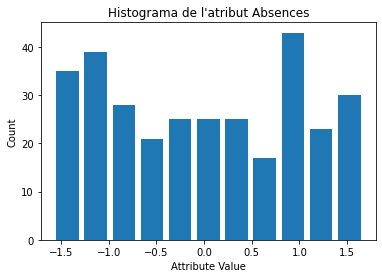
\includegraphics[width=0.3\textwidth]{HISTOGRAMAS/histograma_absences.png}}
  \subfloat[\textit{Department}]{
    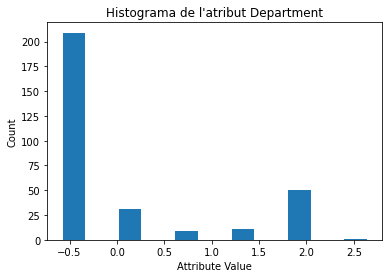
\includegraphics[width=0.3\textwidth]{HISTOGRAMAS/histograma_department.png}}
  \subfloat[\textit{DOB}]{
    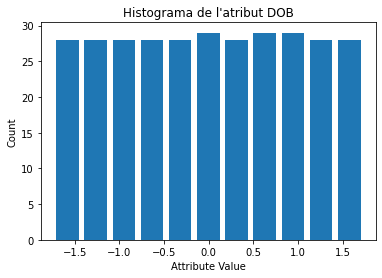
\includegraphics[width=0.3\textwidth]{HISTOGRAMAS/histograma_dob.png}}
 \\
 \centering
  \subfloat[\textit{EmploymentStatus}]{
    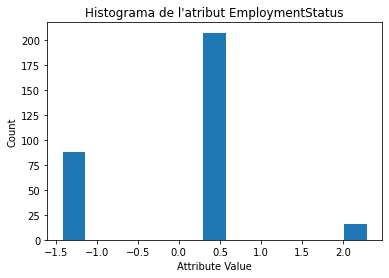
\includegraphics[width=0.3\textwidth]{HISTOGRAMAS/histograma_employmentstatus.png}}
  \subfloat[\textit{ManagerID}]{
    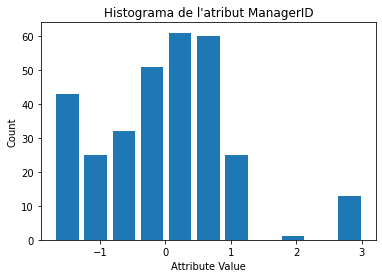
\includegraphics[width=0.3\textwidth]{HISTOGRAMAS/histograma_managerid.png}}
  \subfloat[\textit{Position}]{
    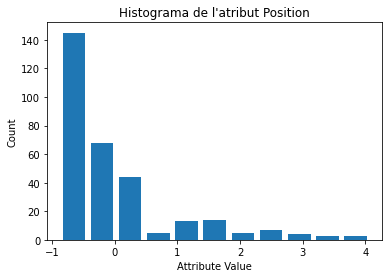
\includegraphics[width=0.3\textwidth]{HISTOGRAMAS/histograma_position.png}}
 \\
 \centering
  \subfloat[\textit{Salary}]{
    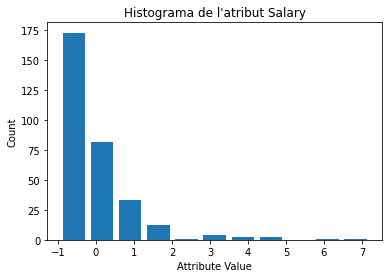
\includegraphics[width=0.3\textwidth]{HISTOGRAMAS/histograma_salary.png}}
  \subfloat[\textit{State}]{
    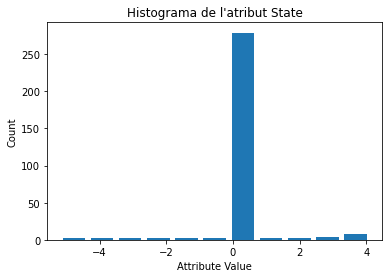
\includegraphics[width=0.3\textwidth]{HISTOGRAMAS/histograma_state.png}}
  \subfloat[\textit{Sex}]{
    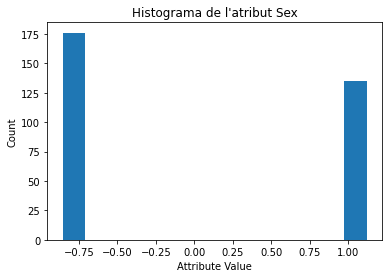
\includegraphics[width=0.3\textwidth]{HISTOGRAMAS/histograma_sex.png}}
    \\
  \caption{Histogrames dels atributs}
\end{figure}
\hspace{-1.8 em}
S'observa dels histogrames\footnote{Es mostren part dels histogrames obtinguts, la resta es troben a \textcolor{blue}{\ref{histograma}}} que cap atribut segueix una distribució normal.\\
La majoria d'atributs segueixen distribucions discretes o uniformes (pel que el seu impacte en la predicció serà poc rellevant o nul).\\\\
Per altra banda, existeixen alguns atributs (com el que volem predir, el \textit{Salary}) que sembla que segueixin una distribució exponencial. S'intentarà utilitzar aquesta informació més endavant per a millorar la nostra predicció.\\\\
\textbf{IMPORTANT:} Els histogrames han sigut fets amb les dades estandaritzades per així poder visualitzar de millor manera com estan distribuïdes les dades, ja que en alguns casos els valors eren molt dispars i es dificultava la interpretació del gràfic.
\newpage
\subsection{Correlació de les variables} \label{correlacio}
Mostrem ara l'anàlisi de les correlacions dels atributs de la base de dades.\\ 
Mencionar que els càlculs de les correlacions han sigut amb el dataset sense estandaritzar.
\begin{figure}[h] % Flotante "comun", sin caption, en que irán ambos
\begin{minipage}{8cm} % Minipagina para la tabla. 8 cm de ancho
\begin{center}
    \begin{tabular}{l|l}
        \textbf{Atribut} & \textbf{\# afins}\\\hline\hline
        Employee\_Name & 10 \\\hline
        EmpID &  4 \\\hline
        MarriedID & 0 \\\hline
        MaritalStatusID & 1 \\\hline
        EmpStatusID & 4 \\\hline
        GenderID & 1  \\\hline
        DeptID & 9  \\\hline
        PerfScoreID & 5   \\\hline
        FromDiveristyJobFairID & 1 \\\hline
        Salary & 10   \\\hline
        Termd & 4\\\hline
        PositionID & 2 \\\hline
        Position & 10 \\\hline
        State &  0 \\\hline
        Zip & 1 \\\hline
        DOB & 10 \\\hline
        Sex & 1 \\\hline
        MaritalDesc & 1\\\hline
        CitizenDesc & 0 \\\hline
        HispanicLatino & 0 \\\hline
        RaceDesc & 1 \\\hline
        DateofHire & 10 \\\hline
        TermReason & 5 \\\hline
        EmploymentStatus & 4 \\\hline
        Department & 10 \\\hline
        ManagerName & 11 \\\hline
        ManagerID & 11 \\\hline
        RecruitmentSource & 0 \\\hline
        PerformanceScore & 2 \\\hline
        EngagementSurvey & 3 \\\hline
        EmpSatisfaction & 1 \\\hline
        SpecialProjectsCounts & 10 \\\hline
        LastPerformanceReview\_Date & 13 \\\hline
        DaysLateLast30 & 3\\\hline
        Absences & 0\\
    \end{tabular}
    Taula 1: Taula d'atributs afins
    \setcounter{table}{1}
    \label{tab:afins}
\end{center}
\end{minipage} % Fin de la minipagina de la tabla
\hspace{2em}
%\hfill % Espacio flexible para separar tabla y figura
\begin{minipage}{6.3cm} % Minipágina para la figura, 4 cm de ancho
\begin{center}
   \begin{tabular}{l|l}
        \textbf{Atribut} & \textbf{Corr.}\\\hline\hline
        Employee\_Name & $0.756$ \\\hline
        Position &  $0.917$ \\\hline
        DOB & $0.751$ \\\hline
        DateofHire & $0.586$ \\\hline
        Department & $0.622$ \\\hline
        ManagerName & $0.654$  \\\hline
        SpecialProjectsCount & $0.508$  \\
\end{tabular}
\captionof{table}{Taula d'atributs rellevants} 
\end{center}
S'observa a la figura 2 mostrada
que alguns dels atributs amb més
relacions són \textit{Employee\_Name},
\textit{Salary}, \textit{Position} i \textit{DOB}, entre
d'altres. S'escull d'entre els
atributs amb més relacions el
\textit{Salary} com a objectiu per fer-ne
l'estudi, ja que és dels pocs que són
continus, numèrics i afins amb
la resta.\\\\
S'observa, a més, que existeix un conjunt nombrós d'atributs amb el mateix nombre de correlacions que \textit{Salary}, i per això s'intueix que estan relacionats entre ells, afirmant així que existeix una forta relació entre l'atribut \textit{Salary} i la resta d'atributs de la base de dades.
\\\\
Per altra banda, s'observa a la
figura 3 la correlació entre
l'atribut \textit{Salary} i la resta
d'atributs del dataset.
Cal recalcar que només es mostren els
atributs que presenten una correlació
major al $0.5$ (els atributs rellevants).
\end{minipage} % Fin de la minipagina que lleva la foto
\end{figure} % Fin del entorno comun. No lleva caption
\newpage
\hspace{-1.7 em}Una vegada reduït el conjunt de dades a analitzar de 36 a 7 atributs, s'estudia si tenen alguna distribució (respecte a la resta) que indiqui alguna duplicitat de les dades o alguna distribució que útil per predir el valor del \textit{Salary}.

\begin{figure}[h]
 \centering
    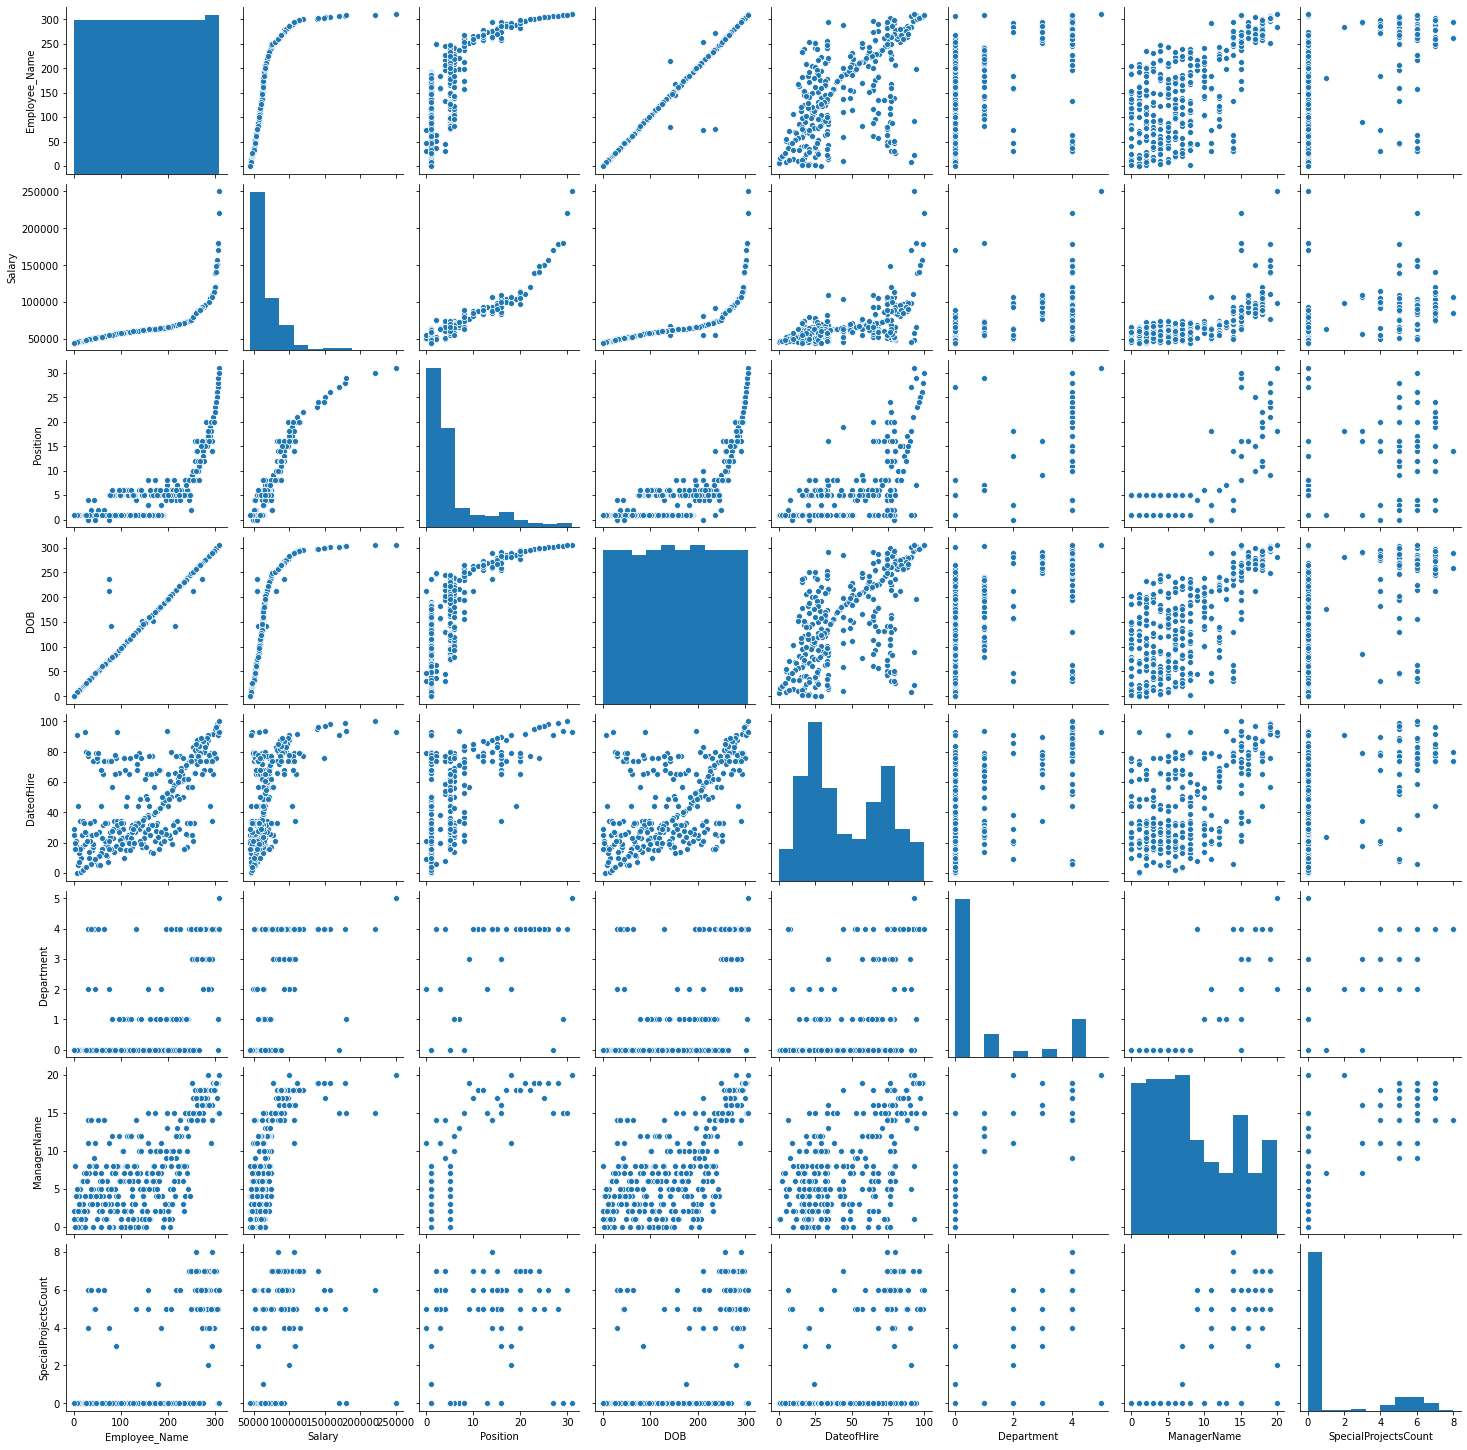
\includegraphics[width=1\textwidth]{CORRELACIONS/grafics_correlacons.png}
    \caption{Pairplot dels atributs rellevants i l'objectiu}
    \label{pairplot}
\end{figure}
\hspace{-1.8 em}
Els gràfics estan ordenats de la següent forma: Employee\_Name, Salary, Position, DOB, DateofHire, Department, ManagerName i SpecialProyectsCount.\\
S'observa com els atributs Employee\_Name, DOB, Position i ManagerName semblen seguir distribució exponencial respecte al Salary.\\
Per altra banda, hi ha atributs com el DateofHire que tot i que sembla tenir alguna relació, té molts valors dispersos.\\
També hi ha atributs com SpecialProyectCount que no es veu a simple vista quina relació hi ha.\\
\\
S'observa com les variables DOB i Employee\_name tenen distribucions uniformes i una relació entre elles massa lineal. Estudiem mitjançant un mapa de calor quina relació hi ha entre elles, entre la resta d'atributs rellevants i entre el Salary.
\newpage 

\begin{figure}
    \centering
    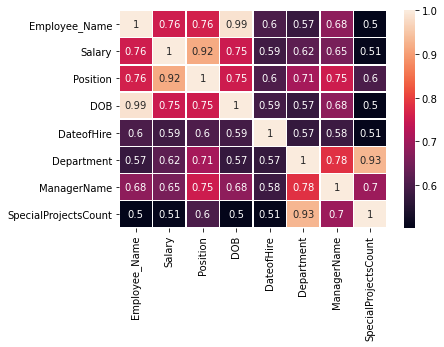
\includegraphics[width=0.8\textwidth]{CORRELACIONS/correlacions.png}
    \caption{Heatmap dels atributs rellevants i l'objectiu}
    \label{fig:my_label}
\end{figure}
\hspace{-1.8 em}
S'observa del mapa de calor que existeix una forta correlació entre totes les dades rellevants.\\
A més, s'observa com el millor atribut (pel que fa a que té la millor correlació amb l'objectiu) és el \textit{Position}.\\\\
Per altra banda, destaca el fet que la correlació entre els atributs \textit{Employee\_Name} i \textit{DOB} és quasi de $1$, encara que no hauria de tenir tanta correlació, ja que en una empresa real amb tants treballadors, el normal és que entre diversos treballadors hi hagués alguns amb el mateix nom i/o la mateixa data de naixement. Es dedueix el següent:
\begin{enumerate}
    \item Tant el \textit{DOB} com l'\textit{Employee\_Name} segueixen distribucions uniformes pel que no es repeteixen ni dates de naixement ni noms en la majoria dels casos.
    \item L'empresa no té suficients treballadors com perquè succeeixi una repetició significativa de les dades de \textit{DOB} i \textit{Name}.
\end{enumerate}
Per aquest fenomen, deduïm que no es pot utilitzar la \textit{DOB} i el \textit{Employee\_Name} per predir el \textit{Salary}.\\\\
Mencionar que el fet que l'empresa sigui fictícia perjudica les prediccions, perquè no permet tenir en compte efectes socials per a predir el \textit{Salary}, com racisme o sexisme, ja que no compleix cap desigualtat que podria patir una empresa real. Per altra banda, representen les dades que hauria de tenir una empresa sense cap "brecha" \hspace{0.05em} salarial a causa de discriminacions, i per això ens dediquem a estudiar les autèntiques bases de tenir un sou més elevat o no: els càrrecs de l'empresa, el treball extra, el coordinador, etc...\\\\
Concloem l'estudi de les correlacions crivant les dades a únicament \textit{Position}, \textit{DateofHire}, \textit{Department}, \textit{ManagerName} i \textit{SpecialProjectsCount}.
\newpage
\subsection{Representació de les dades}
Decidim representar les dades del Salary respecte dels atributs rellevant en R3 per veure si hi existeix alguna relació visual amb el valor del Salary.
\subsubsection{Representació 2 a 2 en R3}\label{representacio2a2}
A l'hora de representar a R3 el Salary respecte de 2 atributs ens adonem que hi ha un conjunt de gràfics on es veu fàcilment una relació i un altre conjunt on no es veu cap relació aparent. Mostrem ara una mostra dels gràfics estudiats\footnote{El conjunt de gràfics complets es troba a \textcolor{blue}{\ref{PCA}}}.\\
En aquest cas, els gràfics s'han fet amb els atributs estandaritzats i el Salary amb els valors originals per a poder enfatitzar el creixement exponencial d'alguns dels gràfics.
\begin{figure}[h]
 \centering
  \subfloat[\hspace{2 em}DateofHire \& Department]{
    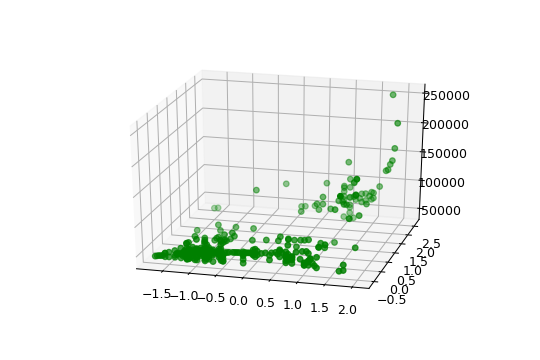
\includegraphics[width=0.5\textwidth]{pca/pca_dateofhire_department.png}}
  \subfloat[\hspace{2 em}ManagerName \& Position]{
    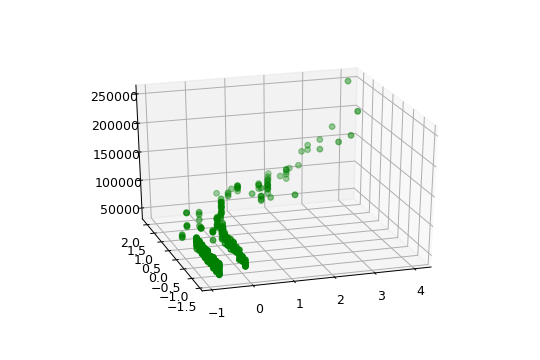
\includegraphics[width=0.5\textwidth]{pca/pca_position_managername.png}}
  \caption{Gràfics amb relacions aparents}
\end{figure}
\begin{figure}[h]
 \centering
   \subfloat[\hspace{2 em}ManagerName \& SpecialProyectCount]{
    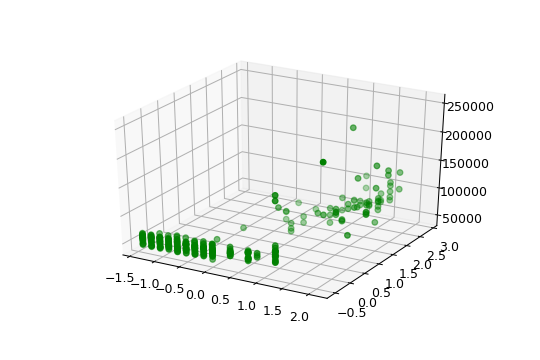
\includegraphics[width=0.5\textwidth]{pca/pca_managername_specialprojectscount.png}}
   \subfloat[\hspace{2 em}Department \& ManagerName]{
    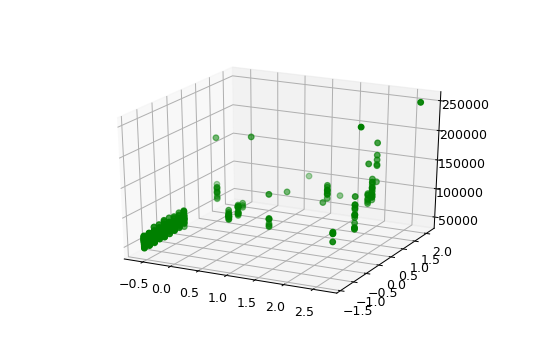
\includegraphics[width=0.5\textwidth]{pca/pca_department_managername.png}}
   \caption{Gràfics sense relacions aparents}
\end{figure}\\
S'observa doncs com sembla que només els atributs DateofHire i Position obtenen alguna relació amb combinació dels altres atributs amb el Salary. \\
Es conclou que per a predir el Salary només és imprescindible  els atributs DateofHire i Position.\\
Es procedeix a estudiar el comportament però en comptes de 2 a 2 fent 3 a 3.
\newpage
\subsubsection{Representació 3 a 3 en R4}
Per a poder representar les dades amb 4 atributs (el Salary i 3 més dels 5 rellevants), s'ha decidit posar el valor de Salary com el color del punt. Cada eix representa un dels atributs.\\
Els atributs estan  estandaritzats, però el Salary està normalitzat (han sigut dividits pel valor màxim que assoleix el Salary) per a evitar que la diferència de colors sigui poc visible.\\
Una mostra dels resultats obtinguts són\footnote{El conjunt de gràfics complets es troba a \textcolor{blue}{\ref{PCA}}}:
\begin{figure}[h]
 \centering
  \subfloat[DateofHire \& Department \& ManagerName]{
    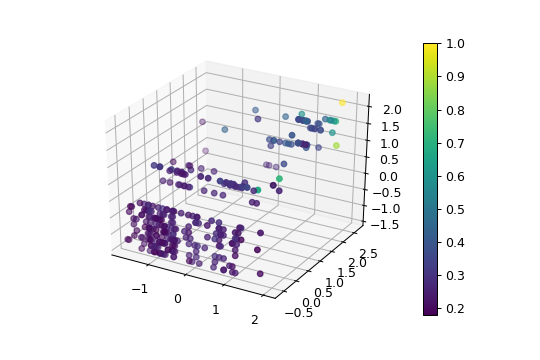
\includegraphics[width=0.5\textwidth]{pca/pca_dateofhire_department_managername.png}}
  \subfloat[DateofHire \& Position \& Department]{
    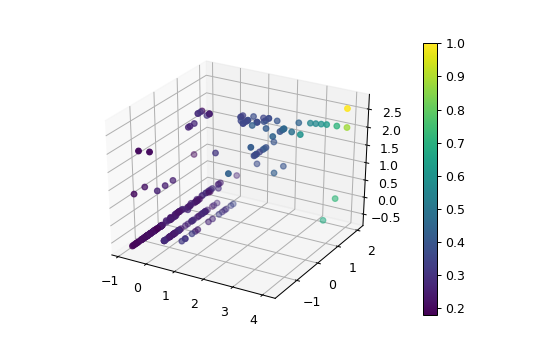
\includegraphics[width=0.5\textwidth]{pca/pca_position_dateofhire_department.png}}
  \caption{Gràfics del Salary amb els atributs 3 a 3 }
 \end{figure}\\
 Dels gràfics ens adonem que no hi existeix cap relació adicional a les ja trobades amb les representacions del Salary fetes anterioemnt a \textcolor{blue}{\ref{pairplot}} i \textcolor{blue}{\ref{representacio2a2}}, i per això deduïm que no hi haurà una gran millora dels resultats una vegada afegim més atributs per al nostre regressor.\\ 
 Igualment s'estudia si la millora que obtenim és considerable o si pel contrari amb un nombre menor de variables s'obté un resultat prou bo.
 \newpage
\section{PCA} \label{PCA}
Per tal de trobar noves relacions que puguin ser significatives a l'hora de predir el \textit{Salary}, es decideix provar d'examinar les dades rellevants mitjançant una PCA.\\\\
Els resultats obtinguts d'aquest analísi és la següent:\\
\begin{figure}[h]
    \centering
    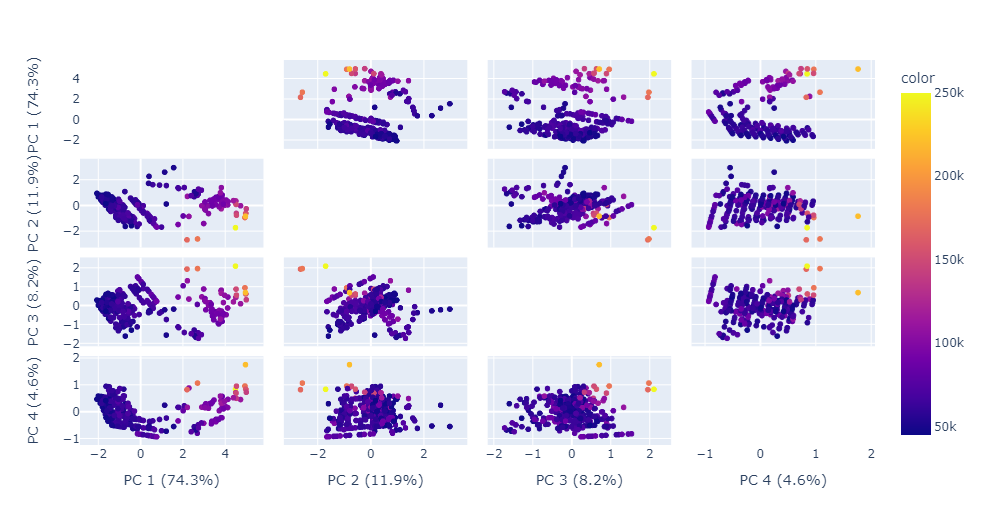
\includegraphics[width=1\textwidth]{pcabona.png}
    \caption{PCA dels atributs rellevant per al Salary}
\end{figure}\\
S'observa de l'analísi de la PCA que cap combinació lineal de variables ens dona una bona variança (millor que la que es podria obtenir mitjançant les variables de forma independent). \\
El millor valor de variança que aconseguim és entre la PC4 i PC1 amb 74.3\%. Aquest valor, tot i ser bastant bo, no entra dins del llindar òptim per a fer una PCA (superior o igual al 85\%)\footnote{El valor del llindar superior a 85\% ha sigut extret en la investigació prèvia a l'ús de la PCA on diverses fonts comenten que en cas d'obtenir una molt bona correlació entre algunes dades amb l'atribut objectiu superior a la variança de la PCA és recomanable no invertir temps en desenvolupar  l'anàlisi de la PCA i millorar la regressió mitjançant les variables de forma independent}.\\\\
Es dedueix, doncs, que es pot obtenir resultats millors utilitzant altres mètodes que no pas una PCA (com per exemple utilitzar transformacions en les dades, fer regressió mitjançant mètodes alternatius, etc.).
\newpage
\section{Predicció del Salary}
Per a predir el \textit{Salary} s'han utilitzat diversos mètodes i transformacions. Primerament, s'ha intentat fer una regressió lineal simple per a totes les dades (incloses les descartades) per si existia alguna relació que havia sigut descuidada.\\\\ Posteriorment s'han procedit a estudiar diversos tipus de regresor que s'han cregut útils per a veure amb quin obtenim la millor predicció.\\\\ Finalment s'ha procedit a fer un interval de confiança per als regressors que s'han cregut necessaris, per a obtenir la millor precisió possible.
\newpage
\subsection{Regressió Lineal}\label{lineal_simple}
Per a trobar el millor regresor lineal estudiem, per als atributs rellevants, el seu MSE i el R2 score.\\\\
S'utilitzen els resultats obtinguts per comparar-los amb altres regresors lineals. \\
Per al regresor lineal simple, s'utilitza el mètode \textit{LinearRegressor()} de la llibreria sklearn\footnote{La informació sobre les llibreries i funcions utilitzades es troba a \textcolor{blue}{\ref{imports}}}.\\\\
\textbf{IMPORTANT:} les dades obtingudes a continuació són mitjançant tots els valors dels que es disposa.
\begin{table}[h]
  \centering
  \begin{tabular}{l||c|c||c|c}
        \multirow{2}{*}{\textbf{Atribut}} & \multicolumn{2}{c||}{\textbf{Original}} & \multicolumn{2}{c}{\textbf{Transformada}}\\
        & MSE & R2 & MSE & R2 \\ \hline \hline
        Position & $100\cdot 10^6$ & $0.841$ & $73\cdot 10^6$ & $0.816$\\\hline
        DateofHire & $414\cdot 10^6$ & $0.343$ & $387\cdot 10^6$ & $0.383$\\\hline
        Department & $387\cdot 10^6$ & $0.387$ & $333\cdot 10^6$ & $0.226$\\\hline
        ManagerName & $361\cdot 10^6$ & $0.428$ & $391\cdot 10^6$ & $0.353$\\\hline
        SpecialProjectsCounts & $468\cdot 10^6$ & $0.258$ & $791\cdot 10^6$ & $0.141$\\
    \end{tabular}
    \caption{MSE i R2 del regressor lineal simple}
    \label{tab:my_label}
\end{table}\\
S'observa com, per a tots els atributs, el MSE és menor quan les dades són estandaritzades, i per això, tot i que el R2 score disminueix  significativament en alguns casos, es decideix utilitzar per a tots els regresors l'estandarització  de les dades.\\\\
\textbf{IMPORTANT:} En aquest cas, com en els següents, les dades estandaritzades són totes menys el \textit{Salary}.\\\\
En cas de fer la regressió i validant-la amb conjunts de train i de test, s'obtenen els següents resultats:
\begin{figure}[h] % Flotante "comun", sin caption, en que irán ambos
\begin{minipage}{8cm} % Minipagina para la tabla. 8 cm de ancho
\begin{center}
    \begin{tabular}{l||c|c}
        \textbf{Atribut} & MSE & R2 \\ \hline \hline
        Position & $81\cdot 10^6$ & 0.857 \\\hline
        DateofHire & $272\cdot 10^6$ & 0.340 \\\hline
        Department & $232\cdot 10^6$ & 0.454 \\\hline
        ManagerName & $194\cdot 10^6$ & 0.539 \\\hline
        SpecialProjectsCounts & $293\cdot 10^6$ & 0.217 \\
    \end{tabular}\\
    \captionof{table}{MSE i R2 amb dataset dividit}
    \label{tab:afins}
\end{center}
\end{minipage} % Fin de la minipagina de la tabla
\hspace{2em}
%\hfill % Espacio flexible para separar tabla y figura
\begin{minipage}{6.3cm} % Minipágina para la figura, 4 cm de ancho
\begin{center}
   \begin{center}
    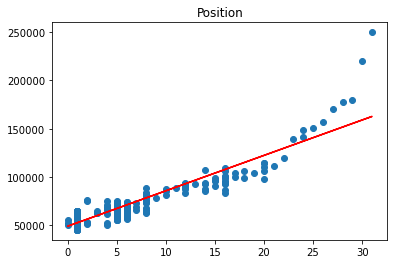
\includegraphics[width=6cm]{REGRESIONS_LINEALS/lineal_position.png}
    % De nuevo usamos capt-of para poner caption en esta parte
    \captionof{figure}{Regressor de Position}
    \label{regresor_lineal_simple}
    \end{center}
\end{center}
\end{minipage} % Fin de la minipagina que lleva la foto
\end{figure} % Fin del entorno comun. No lleva caption
\\
Es conclou doncs que, tot i tenir un error inacceptable, el millor regresor lineal simple és mitjançant l'atribut Position\footnote{La resta de gràfics obtinguts amb el MSE i R2 corresponents per aquesta anàlisi es troben a \textcolor{blue}{\ref{graf_regresion}}}.\\
Es dedueix que aquest error és tant elevant a causa de la gran variança del \textit{Salary} entre els treballadors amb \textit{Positions} de molta i poca importància.\\
Solucionem aquest problema mitjançant transformacions al dataset per, així, obtenir millors precisions.
\newpage
\subsection{Regressió lineal amb escala logarítmica}\label{tranformacio_loaritmica}
Observem de totes gràfiques generades (com per exemple \textcolor{blue}{\ref{pairplot}}, \textcolor{blue}{\ref{representacio2a2}}, \textcolor{blue}{\ref{regresor_lineal_simple}} i les classificades a \textcolor{blue}{\ref{graf_regresion}}) que el valor de l'atribut \textit{Salary} creix de manera exponencial, pel que procedim a fer la regessió lineal de l'apartat anterior (\textcolor{blue}{\ref{lineal_simple}}) però aplicant la transformació logarítmica a les dades del \textit{Salary}:
$$\sum_{i}^{n} w_i x_i = \log y \Longrightarrow y = \exp\left(\sum_{i}^{n} w_i x_i\right)$$
Mitjançant aquest nou model recalculem el MSE i el R2 score de les variables més rellevants\footnote{El conjunt sencer dels gràfics es troben a \textcolor{blue}{\ref{regressio_lineal_simple_log}}}.
\begin{figure}[h] % Flotante "comun", sin caption, en que irán ambos
\begin{minipage}{8cm} % Minipagina para la tabla. 8 cm de ancho
\begin{center}
    \begin{tabular}{l||c|c}
        \textbf{Atribut} & MSE & R2 \\ \hline \hline
        Position & $0.010$ & 0.862 \\\hline
        DateofHire & $0.045$ & 0.404 \\\hline
        Department & $0.042$ & 0.440 \\\hline
        ManagerName & $0.036$ & 0.520 \\\hline
        SpecialProjectsCounts & $0.051$ & 0.321 \\
    \end{tabular}\\
    \captionof{table}{MSE i R2 amb dataset dividit}
    \label{tab:afins}
\end{center}
\end{minipage} % Fin de la minipagina de la tabla
\hspace{2em}
%\hfill % Espacio flexible para separar tabla y figura
\begin{minipage}{6.3cm} % Minipágina para la figura, 4 cm de ancho
\begin{center}
   \begin{center}
    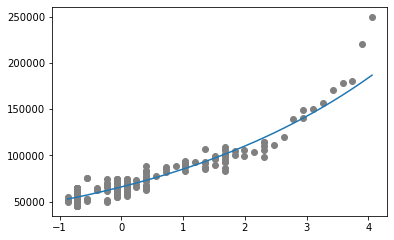
\includegraphics[width=6cm]{Regressor lineal logaritmo/logaritmica_position.png}
    % De nuevo usamos capt-of para poner caption en esta parte
    \captionof{figure}{Regressor de Position}
    \label{regresor_lineal_simple}
    \end{center}
\end{center}
\end{minipage} % Fin de la minipagina que lleva la foto
\end{figure} % Fin del entorno comun. No lleva caption
\\
S'observa una millora notòria  tant en l'error comès  com en l'R2 score a l'hora de predir el valor del \textit{Salary}.\\
\\
Com totes les variables tenen relació exponencial amb \textit{Salary}, aplicarem la transformació logarítmica a tots els nostres regresors per així obtenir una millor predicció.\\\\
A partir d'ara el valor amb el que compararem els resultats següents serà:
\begin{itemize}
    \item MSE\footnote{\textbf{IMPORTANT:} El càlcul de l'error y R2 score s'ha efectuat amb el valor predit, el logaritme de y, no amb $e^y$, on $y$ és el valor predit.}: 0.01
    \item R2 score: 0.862
\end{itemize}
Per mirar de millorar la predicció, provem altres tipus de regresors, com la \textit{BayesianRidge} o \textit{Lasso}.
\newpage
\subsection{Regressió Lineal amb BayessianRidge}
Procedim a estudiar els resultats obtinguts per al mètode de regressió lineal del \\ \textit{BayesianRidge()}\footnote{S'ha introduït com a paràmetre d'entrada $t = 1\cdot 10^{-12}$, on $t$ és la tolerància.} i comparant-los amb els valors anteriorment obtinguts.
\begin{figure}[h] % Flotante "comun", sin caption, en que irán ambos
\begin{minipage}{8cm} % Minipagina para la tabla. 8 cm de ancho
\begin{center}
    \begin{tabular}{l||c|c}
        \textbf{Atribut} & MSE & R2 \\ \hline \hline
        Position & $0.010$ & 0.862 \\\hline
        DateofHire & $0.045$ & 0.404 \\\hline
        Department & $0.042$ & 0.440 \\\hline
        ManagerName & $0.036$ & 0.520 \\\hline
        SpecialProjectsCounts & $0.051$ & 0.321 \\
    \end{tabular}\\
    \captionof{table}{MSE i R2 amb dataset dividit}
    \label{tab:afins}
\end{center}
\end{minipage} % Fin de la minipagina de la tabla
\hspace{2em}
%\hfill % Espacio flexible para separar tabla y figura
\begin{minipage}{6.3cm} % Minipágina para la figura, 4 cm de ancho
\begin{center}
   \begin{center}
    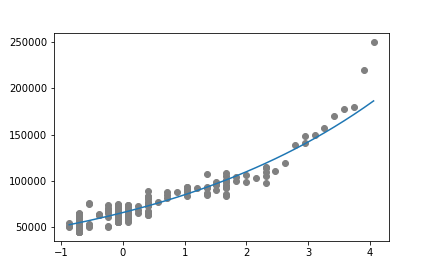
\includegraphics[width=6cm]{bayes/bayes_lineal_position.png}
    % De nuevo usamos capt-of para poner caption en esta parte
    \captionof{figure}{Regressor de Position}
    \label{regresor_lineal_simple}
    \end{center}
\end{center}
\end{minipage} % Fin de la minipagina que lleva la foto
\end{figure} % Fin del entorno comun. No lleva caption
\\
S'observa dels resultats obtinguts que no existeix cap diferència (en els primers tres decimals) en les dades obtingudes  amb el regresor lineal simple. \\
Es conclou doncs que el model anterior es manté com el millor per a predir el \textit{Salary}.
\\\\\\
\subsection{Regressió lineal amb Lasso}\label{lineal_lasso}
Es procedeixen a estudiar els resultats obtinguts per al mètode de regressió lineal del \\ \textit{Lasso()}\footnote{S'ha introduït com a paràmetre d'entrada $a = 0.001$, on $a$ és el terme de regularització.} i comparant-los amb els valors anteriorment obtinguts.
\begin{figure}[h] % Flotante "comun", sin caption, en que irán ambos
\begin{minipage}{8cm} % Minipagina para la tabla. 8 cm de ancho
\begin{center}
    \begin{tabular}{l||c|c}
        \textbf{Atribut} & MSE & R2 \\ \hline \hline
        Position & $0.010$ & 0.862 \\\hline
        DateofHire & $0.045$ & 0.404 \\\hline
        Department & $0.042$ & 0.440 \\\hline
        ManagerName & $0.036$ & 0.520 \\\hline
        SpecialProjectsCounts & $0.051$ & 0.321 \\
    \end{tabular}\\
    \captionof{table}{MSE i R2 amb dataset dividit}
    \label{tab:afins}
\end{center}
\end{minipage} % Fin de la minipagina de la tabla
\hspace{2em}
%\hfill % Espacio flexible para separar tabla y figura
\begin{minipage}{6.3cm} % Minipágina para la figura, 4 cm de ancho
\begin{center}
   \begin{center}
    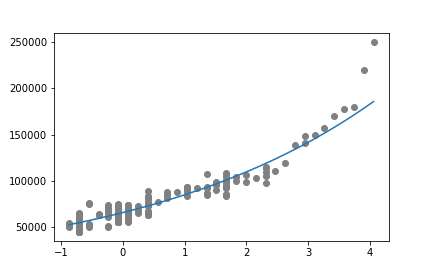
\includegraphics[width=6cm]{lasso/lasso_lineal_position.png}
    % De nuevo usamos capt-of para poner caption en esta parte
    \captionof{figure}{Regressor de Position}
    \label{regresor_lineal_simple}
    \end{center}
\end{center}
\end{minipage} % Fin de la minipagina que lleva la foto
\end{figure} % Fin del entorno comun. No lleva caption
\\
S'observa dels resultats obtinguts que no existeix cap diferència (en els primers 3 decimals) en les dades obtingudes  amb el regresor lineal simple. \\
Es conclou doncs que el model anterior es manté com el millor per a predir el \textit{Salary}.\\\\
Tot i això, s'ha decidit que és millor utilitzar el mètode \textit{Lasso()} ja que permet escollir el grau de precisió de la recta de regressió mitjançant el paràmetre $a$\footnote{Mencionar que s'ha estudiat que a partir del valor $a\leq 0.01$, el regressor només estabilitza els valors, no augmenta significativament la precisió.} i calcula les rectes de regressió més ràpid que el regresor simple.\\\\
\newpage
\subsection{Regressió multilineal}
Es procedeix ara a intentar millorar la precisió del regresor afegint-li major complexitat. S'analitzen ara, totes les possibles combinacions lineals del regressor multilineal simple de la llibreria sklearn (\textit{LinearRegressor()}) amb totes les variables rellevants\footnote{Per a fer aquestes combinacions s'ha utilitzat el mètode explicat a \textcolor{blue}{\ref{combination}}}.\\\\
Els resultats més significatius obtinguts\footnote{La resta de resultats obtinguts es troben a \textcolor{blue}{\ref{reg_multi}}}, són els següents:
\begin{table}[h]
    \centering
    \begin{tabular}{c||c|c}
        \cellcolor{white}{} & Atributs & Valor \\ \hline \hline
        Millor R2 & Position, DateofHire, Department & 0.827 \\ \hline
        Millor MSE & Position, DateofHire, ManagerName & $102\cdot 10^6$
    \end{tabular}
    \caption{Millors valors de MSE i R2 obtinuts en la regressió multilineal}
    \label{tab:my_label}
\end{table}\\Abans d'explicar els resultats cal comentar que els estudis del regresor multilineal s'han dut a terme amb els datatset separat en train i test i que s'han repetit els càlculs 1000 vegades per cada conjunt d'atributs trobats per a evitar valors sobre o infraestimats deguts a fenòmens aleatoris i evitar també possibles overfittings del model.\\\\
S'observa com tant l'error MSE com el R2 score no milloren significativament respecte a la millor combinació trobada fins al moment.\\
Tot i això, es pot observar una certa millora respecte a la mitjana de valors obtiguts inicialment.\\\\
Es conclou que el mètode de regressió multilineal pot superar en precissió al millor regresor trobat fins ara, per això es decideix aplicar una transformació al datatset per així intentar millorar la predicció.
\subsection{Regressió multilineal amb escala logarítmica}
Repetim ara la mateixa transformació que en l'apartat \textcolor{blue}{\ref{tranformacio_loaritmica}} per a veure si el regresor multilineal simple és capaç de millorar l'error comès.\\
Els resultats més significatius obtinguts\footnote{La resta de resultats obtinguts es troben a \textcolor{blue}{\ref{reg_multi_log}}}, són els següents:
\begin{table}[h]
    \centering
    \begin{tabular}{c||c|c}
        \cellcolor{white}{} & Atributs & Valor \\ \hline \hline
        Millor R2 & Position, DateofHire, ManagerName & 0.857 \\ \hline
        Millor MSE & Position, DateofHire & $0.010$
    \end{tabular}
    \caption{Millors valors de MSE i R2 obtinuts en la regressió multilineal}
    \label{tab:my_label}
\end{table}\\
S'observa com tant l'error com el R2 score no arriben a millorar, però si quasi igualar completament, els valors obtinguts pel millor regresor fins ara.\\
Com hi ha hagut una millora molt significativa respecte al regressor multilineal simple, procedim a intentar millorar els valors obtinguts pel regresor estudiant diferents mètodes.\\\\
Cal mencionar que ha aparegut una discrepància entre els atributs trobats a l'apartat anterior i aquest, aquest fenomen segurament és a causa de que els atributs trobats aquesta vegada són en els que la tendència exponencial està més present.
\newpage
\subsection{Regressió multilineal amb Lasso}
Estudiem ara els millors valors assolits de totes les combinacions d'atributs rellevants mitjançant el mètode de regressió multilineal \textit{Lasso()}\footnote{Igual que en seu anàleg lineal el valor del paràmetre $a = 0.01$}.\\
Com els resultats obtinguts per la transformació han millorat el regresor lineal, utilitzem la transformació per al regresor multilineal amb mètode \textit{Lasso()}.
\\
Els resultats més significatius obtinguts\footnote{La resta de resultats obtinguts es troben a \textcolor{blue}{\ref{reg_multi_lasso}}}, són els següents:
\begin{table}[h]
    \centering
    \begin{tabular}{c||c|c}
        \cellcolor{white}{} & Atributs & Valor \\ \hline \hline
        Millor R2 & Position, DateofHire, ManagerNamee & 0.716 \\ \hline
        Millor MSE & Position, DateofHire, Department, ManagerName & $0.020$
    \end{tabular}
    \caption{Millors valors de MSE i R2 obtinuts en la regressió multilineal Lasso}
    \label{tab:my_label}
\end{table}\\
S'observa com el regresor multilineal amb mètode Lasso no millora ni en R2 ni en MSE al regresor multilineal simple, per la qual cosa s'intenta millorar la precisió amb un altre mètode.
\subsection{Regressió multilineal amb BayessianRidge}
Estudiem ara els millors valors obtinguts de totes les combinacions d'atributs rellevants mitjançant el mètode de regressió multilineal \textit{BayessianRidge()}\footnote{Igual que en seu anàleg lineal el valor del paràmetre $t = 10^{-12}$}.\\
Com els resultats obtinguts per la transformació han millorat el regresor lineal, utilitzem la transformació per al regresor multilineal amb mètode \textit{BayessianRidge()}.
\\
Els resultats més significatius obtinguts\footnote{La resta de resultats obtinguts es troben a \textcolor{blue}{\ref{reg_multi_bay}}}, són els següents:
\begin{table}[h]
    \centering
    \begin{tabular}{c||c|c}
        \cellcolor{white}{} & Atributs & Valor \\ \hline \hline
        Millor R2 & Position, DateofHire & $0.857$ \\ \hline
        Millor MSE & Position, DateofHire & $0.010$
    \end{tabular}
    \caption{Millors valors de MSE i R2 obtinuts en la tilineal BayessianRidge}
    \label{tab:my_label}
\end{table}\\
S'observa com, mitjançant el mètode \textit{BayessianRidge()}, els millors valors de MSE i R2 score coincideixen en els dos casos amb el mateix conjunt d'atributs.\\\\
Comentar també que són els dos millors atributs dels rellevants (com ja hem estudiat a \textcolor{blue}{\ref{representacio2a2}}).\\\\
Deduïm d'això que els mètodes multilineals intenten assemblar-se al mètode lineal dels atributs Position i DateofHire (sobretot al del Position) incloent-ne algun d'aquests atributs en el seu model de regressió lineal per així asegurar-se tenir una bona predicció.\\\\
Com que cap dels regressors ha siguit capaç de superar en R2 score o en MSE al regresor de l'apartat \textcolor{blue}{\ref{lineal_lasso}} (Regresor lineal amb mètode Lasso basat en l'aribut Position), es finalitza l'estudi analitzant i polint aquest regresor lineal.
\newpage
\subsection{Versió final del regresor i interval de confiança}
Per finalitzar l'estudi dels regresors, es procedeix a estudiar quin és el marge d'error del nostre regresor i estudiar el seu interval de confiança.\\\\
Calculant l'interval de confiança del 75\%, s'obté el següent llindar:
\begin{figure}[h]
\captionsetup[subfigure]{labelformat=empty}
\centering
  \subfloat[Regressió amb datatset separat en train i test]{
    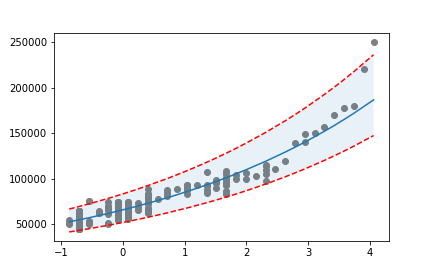
\includegraphics[width=0.5\textwidth]{regressor/75_con_split_regression.png}}
  \subfloat[Regressió sense datatset separat en train i test]{
    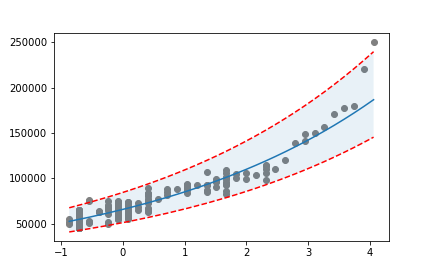
\includegraphics[width=0.5\textwidth]{regressor/75_sin_split_regression.png}}
   \caption{Gràfic de la regressió lineal amb interval de confiança del 75\%}
\end{figure}\\
S'observa com els intervals de confiança tant amb el datatset separat en train i test com sense separar-lo són pràcticament idèntics. \\\\
S'observa com existeixen dos valors (punts) que podrien ser considerats outliners. Aquests es troben a la part superior dreta del gràfic i fa que el regresor augmenti l'error.\\
Els dos outliners representen el \textit{Salary} dels directors de l'empresa (els CEO).\\\\
Com que els sous dels directors de l'empresa és un tema subjecte a canvis, té una dispersió respecte a la resta de dades molt gran i és poc probable de ser necessària de catalogar (ja que en aquest cas es tracta de dos subjectes respecte als 309 restants) es decideix tractar-los com a outliners i eliminar-los per a fer la regresió i l'interval de confiança.\\\\
Mostrem ara el regressor sense els outliners i augmentat l'interval de confiança al 95\%.
\vspace{-1em}
\begin{figure}[h] % Flotante "comun", sin caption, en que irán ambos
\begin{minipage}{7cm} % Minipagina para la tabla. 8 cm de ancho
\begin{center}
    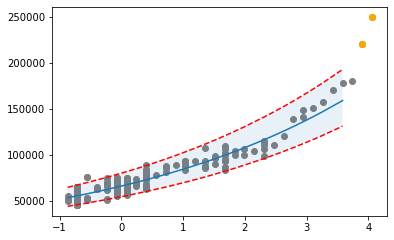
\includegraphics[width=7cm]{lasso/95posicion_sin_outliner_regression.png}
    % De nuevo usamos capt-of para poner caption en esta parte
    \captionof{figure}{Regressor sense outliners amb interval de confiança del 95\%}
    \label{regresor_lineal_simple}
\end{center}
\end{minipage} % Fin de la minipagina de la tabla
\hspace{2em}
%\hfill % Espacio flexible para separar tabla y figura
\begin{minipage}{7cm} % Minipágina para la figura, 4 cm de ancho
\begin{justify}
S'observen en taronja els outliners que no s'han tingut en compte per a fer la regressió lineal, que, com són els últims valors de la gràfica, fa que la regressió s'estanqui quan s'arriba a ells.\\
Tot i això, s'observa com la tendència de la gràfica s'ajusta molt millor als punts que amb els outliners.
\\
També s'observa clarament que tot i haver augmentat l'interval de confiança, aquest sembla haver-se reduït.
\\
Els resultats que s'obtenen (de MSE i R2 score) són 0.007 i 0.880 (respectivament).

\end{justify}
\end{minipage} % Fin de la minipagina que lleva la foto
\end{figure} % Fin del entorno comun. No lleva caption
\newpage 


\section{Resolució de les preguntes}
\subsection{Apartat C}
\begin{enumerate}
    \item \textbf{Quin és el tipus de cada atribut?}\\
    Es pot veure el tipus de cada atribut del dataset a la secció \textcolor{navy}{\ref{tipus_dades}} explicada anteriorment.
    On indica els tres tipus d'atributs que hi ha.
    \item \textbf{Quins atributs tenen una distribució Gaussiana?}\\
    Mitjançant un estudi visual de les gràfiques ,tant a la secció \textcolor{navy}{\ref{distribucions}} com a la \textcolor{navy}{\ref{annex}}, s'ha observat que cap dels atributs dels quals disposa el dataset es pot aproximar per una distribució Gaussiana, tot i que, com s'ha explicat anteriorment, sí que s'observen algunes distribucions uniformes i logarítmiques, entre d'altres.
    \item \textbf{Quin és l'atribut objectiu? Per què?}\\
    S'ha decidit que l'atribut a predir sigui \textit{Salary}, ja que en fer l'estudi de les correlacions entre els atributs mostrat a l'apartat \textcolor{navy}{\ref{correlacio}}, es va veure que és l'atribut amb més correlacions rellevants (sense tenir poca dispersió). Recalcar també que ens semblava dels més interessants a predir, ja que es treballa en el context d'una empresa fictícia.
\end{enumerate}


\newpage
\subsection{Apartat B}
\begin{enumerate}
    \item \textbf{Quins són els atributs més importants per fer una bona predicció?}\\
    S'observa dels gràfics que les millors regressions lineals són amb les variables ja catalogades com a rellevants en l'apartat C: \textit{DateofHire}, \textit{Department}, \textit{Position}, \textit{ManagerName} i \textit{SpecialProjectsCount} (ja que són les que presenten un menor MSE i major R2 score).
    \item \textbf{Amb quin atribut s'assoleix un MSE menor?}\\
    La millor dada obtinguda pel que fa a la relació MSE-R2 és la de \textit{Position}, que, sense estandaritzar, té un MSE = $100190785.86004272$ i R2 = $0.8411741038500034$. Estandaritzat, l'MSE es redueix a $73\cdot 10^6$. 
    \\
    Cal recalcar que en la regressió amb les dades normalitzades s'obtenen un MSE i un R2 bastant més petit i gran respectivament, de manera que els valors que obtenim són més fàcils de tractar.

    \item \textbf{Quina correlació hi ha entre els atributs de la vostra base de dades?
}\\
    Les correlacions de l'atribut \textit{Salary} amb els cinc atributs més rellevants són les següents:

\begin{table}[h]
    \centering
    \begin{tabular}{l|r}
        \textbf{Atribut} & \textbf{Correlació}\\\hline\hline
        Position & 0.917  \\\hline
        DateofHire & 0.586  \\\hline
        Department & 0.622  \\\hline
        ManagerName & 0.654  \\\hline
        SpecialProjectsCount & 0.508 \\
    \end{tabular}
    \label{tab:my_label}
\end{table}\\


    
    \item \textbf{Com influeix la normalització en la regressió?}\\
    En el cas del nostre dataset, ens permet tenir uns valors més "manejables", facilitant la visualització de les dades, les relacions entre elles i detectar les distribucions que segueixen. 

    \item \textbf{Com millora la regressió quan es filtren aquells atributs de les mostres que no contenen informació?}

    Veiem que es redueix l'MSE significativament, mentre que augmenta l'R2 score. Observem que inicialment, usant els 5 atributs més rellevants, s'aconsegueix un error de $75\cdot 10^5$, mentre que usant 3 dels atributs (Position, DateofHire i ManagerName), es redueix a $65\cdot 10^5$. Per altra banda, l'R2 score augmenta de $0.850$ a $0.857$. D'aquesta manera millorem la precisió amb la que el regresor predirà el valor objectiu \textit{Salary}.
    

    \item \textbf{Si s'aplica un PCA, a quants components es redueix l'espai? Per què?}\\
    En fer l'estudi aplicant un PCA, com s'ha explicat a la secció \textcolor{navy}{\ref{PCA}}, observem que la màxima variança que són capaços d'explicar els components principals és de tan sols un $74.3\%$. Decidim així que de totes les combinacions possibles amb els cinc atributs més rellevants, la millor és utilitzant els atributs 'Position', 'DateofHire' i 'ManagerName', ja que és la que presenta una millor relació MSE-R2 score. 

\end{enumerate}


\newpage
\subsection{Apartat A}
\subsubsection{Explicació del regressor lineal programat}
S'ha programat un regresor lineal que està capacitat per a calcular relacions lineals i multilineals\footnote{Per a obtenir més informació sobre el nostre regressor accedir a les últimes cel·les del codi adjuntat conjuntament amb aquesta memòria.}.\\\\
Si bé és funcional i ens permet calcular paràmetres de funcions concretes que poden ser útils per al nostre regresor, el cas és que a causa de com esta organitzat el nostre datatset, és completament inecessari i (inclòs) obté major error que amb els mètodes utilitzats de la llibreria \textit{sklearn}.\\\\
Per aquest motiu no s'ha utilitzat el nostre regresor personalitzat i s'ha prioritzat millorar els regresors dels que ja hi disposàvem.\\\\
Per a observar alguns dels resultats obtinguts pel nostre regresor amb datasets aleatòris accedir a \textcolor{blue}{\ref{descens_gradient}}.

\newpage
\section{Anàlisi i conclusions}
Resumim els resultats obtinguts del nostre estudi:
\begin{itemize}
    \item Com que el dataset ha sigut creat de forma fictícia i no conté informació real, hi apareixen moltes incongruències i dificultats a l'hora d'estimar els valors del \textit{Salary}, per aquests motius mètodes com PCA no són prou bons trobant relacions amb combinacions d'atributs.
    \item Per solucionar el problema anterior s'ha hagut d'estudiar a fons el dataset per a trobar correlacions entre variables i millorar-les per a obtenir bones prediccions. S'ha conclòs que els millors atributs per a fer la regressió eren \textit{Position}, \textit{DateofHire}, \textit{Department}, \textit{SpecialProyectsCount} i \textit{ManagerName}.
    \item Per millorar la predicció dels regresors s'ha optat per fer una transformació logarítmica de les dades i calcular la recta i les prediccions amb aquesta transformació.
    \item S'han provat diferents tipus de regresors (tant lineals com multilineals) per a poder trobar la millor regressió. Es conclou que el millor regresor és el Lasso lineal amb la transformada logarítmica predint el \textit{Salary} mitjançant l'atribut \textit{Position}.
    \item S'ha afegit un interval de confiança del 95\% de confiança eliminant els outliners més significatius del conjunt de dades per, així, millorar encara més la predicció.
\end{itemize}
\begin{figure}[h]
    \centering
    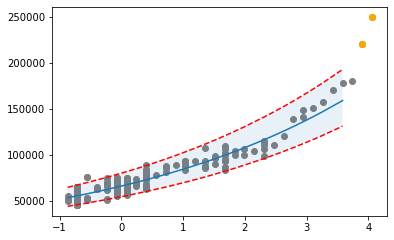
\includegraphics{lasso/95posicion_sin_outliner_regression.png}
    \caption{Gràfic del mètode Lasso, amb transformació logarítmica sense outliners i amb variable independent estandaritzada, amb interval de confiança del 95\%.}
    \label{fig:my_label}
\end{figure}
El nostre regesor per a predir el \textit{Salary} en funció de l'atribut \textit{Position} és:
$$\hat{y} = e^{0.24936\cdot x +11.095}$$
On $\hat{y}$ és la predicció del \textit{Salary} i $x$ és el valor de l'atribut \textit{Position}\footnote{Per a obtenir el valor de la posició es pot utilitzar el diccionari que es genera en la funció \textcolor{blue}{\ref{ordenar_salary}}} després de normalitzar-lo mitjançant la funció \textcolor{blue}{\ref{standariza}}. \\\\
Sabent que un valor d'1 indica un ajust perfecte i, per tant, un model molt fiable per a predir, mentre que un valor de 0 indicaria que el model no aconsegueix ajustar les dades en absolut, assegurem que el nostre regresor funciona de manera correcta comparant la correlació \textit{Salary-Position} ($0.92$), amb l'R2 Score màxim aconseguit, $0.917$.




\newpage
\section{Annex}\label{annex}
\subsection{Histogrames} \label{histograma}
S'adjunten a continuació els histogrames restants mencionats i explicats anteriorment a la secció \textcolor{navy}{\ref{distribucions}}.
\begin{figure}[h]
\captionsetup[subfigure]{labelformat=empty}
 \centering
  \subfloat[\hspace{2 em}CitizenDesc]{
    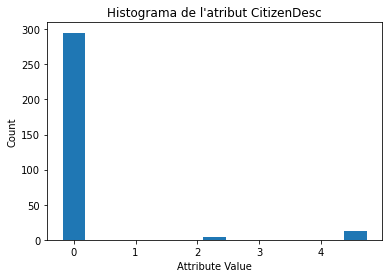
\includegraphics[width=0.3\textwidth]{HISTOGRAMAS/histograma_citizendesc.png}}
  \subfloat[\hspace{2 em}DateofHire]{
    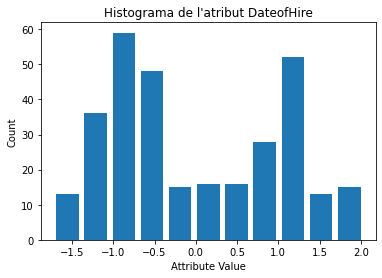
\includegraphics[width=0.3\textwidth]{HISTOGRAMAS/histograma_dateoffire.png}}
  \subfloat[\hspace{2 em}DaysLateLast30]{
    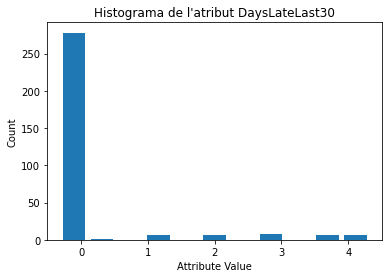
\includegraphics[width=0.3\textwidth]{HISTOGRAMAS/histograma_dayslatelast30.png}}
\end{figure}
\begin{figure}[h]
\captionsetup[subfigure]{labelformat=empty}
\centering
 \subfloat[\hspace{2 em}DeptID]{
    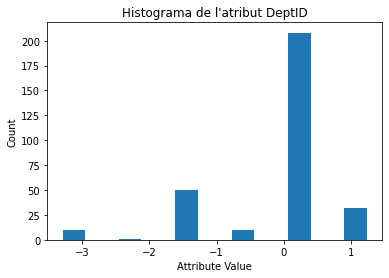
\includegraphics[width=0.3\textwidth]{HISTOGRAMAS/histograma_deptid.png}}
  \subfloat[\hspace{2 em}FromDiversityJobFairID]{
    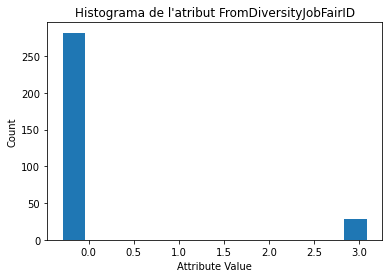
\includegraphics[width=0.3\textwidth]{HISTOGRAMAS/histograma_diversityjob.png}}
  \subfloat[\hspace{2 em}EmpID]{
    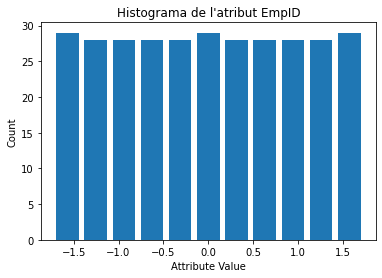
\includegraphics[width=0.3\textwidth]{HISTOGRAMAS/histograma_Emp_id.png}}
\end{figure}
\begin{figure}[h]
\captionsetup[subfigure]{labelformat=empty}
\centering
  \subfloat[\hspace{2 em}Employee\_Name]{
    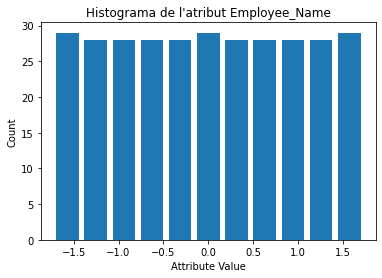
\includegraphics[width=0.3\textwidth]{HISTOGRAMAS/histograma_employee_name.png}}
  \subfloat[\hspace{2 em}EmpSatisfaction]{
    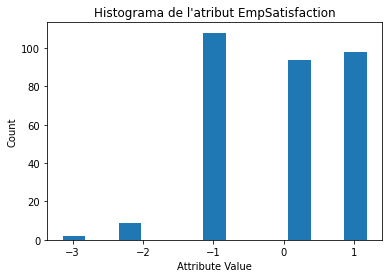
\includegraphics[width=0.3\textwidth]{HISTOGRAMAS/histograma_empsatisfaction.png}}
  \subfloat[\hspace{2 em}EmpStatusID]{
    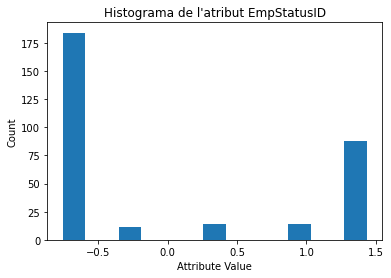
\includegraphics[width=0.3\textwidth]{HISTOGRAMAS/histograma_empstatusid.png}}
\end{figure}
\newpage
\begin{figure}[h]
\captionsetup[subfigure]{labelformat=empty}
\centering
  \subfloat[\hspace{2 em}EngagementSurvey]{
    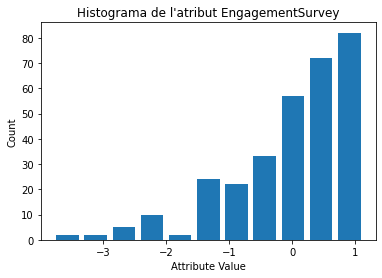
\includegraphics[width=0.3\textwidth]{HISTOGRAMAS/histograma_engagementsurvey.png}}
  \subfloat[\hspace{2 em}GenderID]{
    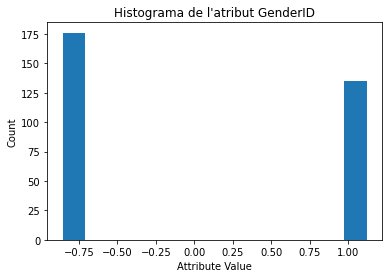
\includegraphics[width=0.3\textwidth]{HISTOGRAMAS/histograma_genderid.png}}
  \subfloat[\hspace{2 em}HispanicLatino]{
    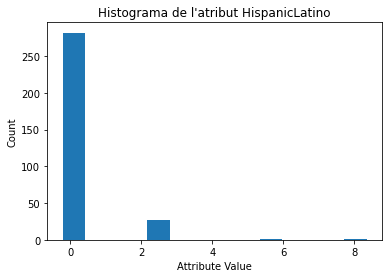
\includegraphics[width=0.3\textwidth]{HISTOGRAMAS/histograma_hispaniclatino.png}}
\end{figure}
\begin{figure}[h]
\captionsetup[subfigure]{labelformat=empty}
\centering
\captionsetup[subfigure]{labelformat=empty}
\centering
  \subfloat[\hspace{2 em}LastPerformanceReview]{
    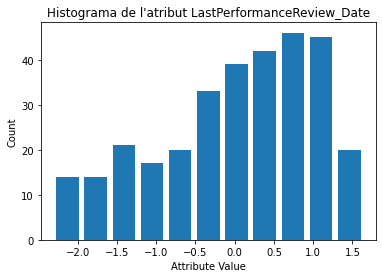
\includegraphics[width=0.3\textwidth]{HISTOGRAMAS/histograma_lastperformancereviewdaate.png}}
  \subfloat[\hspace{2 em}ManagerName]{
    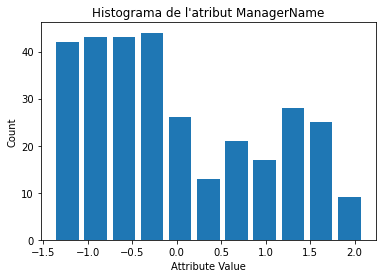
\includegraphics[width=0.3\textwidth]{HISTOGRAMAS/histograma_managername.png}}
  \subfloat[\hspace{2 em}MaritalDesc]{
    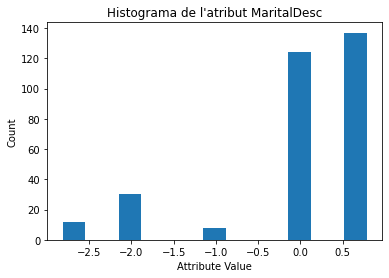
\includegraphics[width=0.3\textwidth]{HISTOGRAMAS/histograma_maritacdesc.png}}
\end{figure}
\begin{figure}[h]
\captionsetup[subfigure]{labelformat=empty}
\centering
  \subfloat[\hspace{2 em}MaritalStatusID]{
    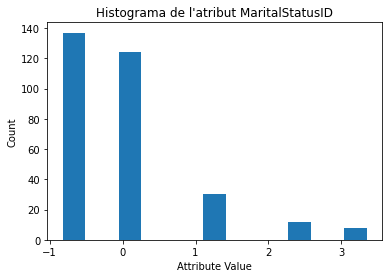
\includegraphics[width=0.3\textwidth]{HISTOGRAMAS/histograma_marital_status.id.png}}
  \subfloat[\hspace{2 em}MarriedID]{
     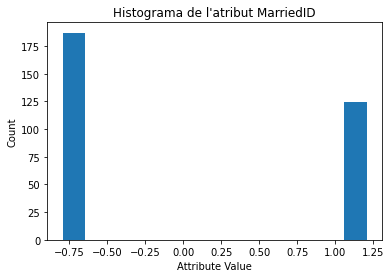
\includegraphics[width=0.3\textwidth]{HISTOGRAMAS/histograma_marriedid.png}}
   \subfloat[\hspace{2 em}PerformanceScore]{
    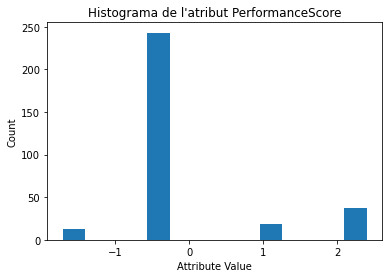
\includegraphics[width=0.3\textwidth]{HISTOGRAMAS/histograma_performancescore.png}}
\end{figure}
\newpage
\begin{figure}[h]
\captionsetup[subfigure]{labelformat=empty}
\centering
  \subfloat[\hspace{2 em}PerfScoreID]{
    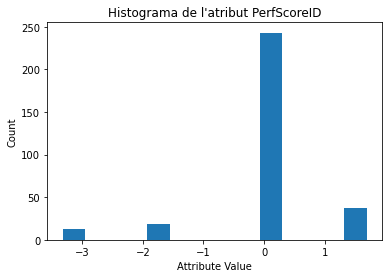
\includegraphics[width=0.3\textwidth]{HISTOGRAMAS/histograma_perfscoreid.png}}
  \subfloat[\hspace{2 em}PositionID]{
    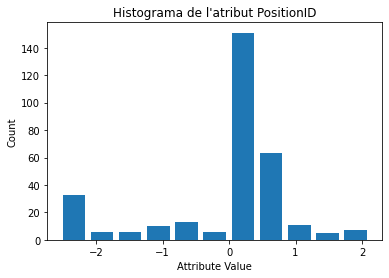
\includegraphics[width=0.3\textwidth]{HISTOGRAMAS/histograma_positionid.png}}
   \subfloat[\hspace{2 em}RecruitmentSource]{
    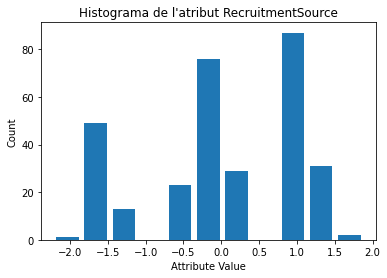
\includegraphics[width=0.3\textwidth]{HISTOGRAMAS/histograma_recruitmentsource.png}}
\end{figure}
\begin{figure}[h]
\captionsetup[subfigure]{labelformat=empty}
\centering
  \subfloat[\hspace{2 em}SpecialProjectsCount]{
    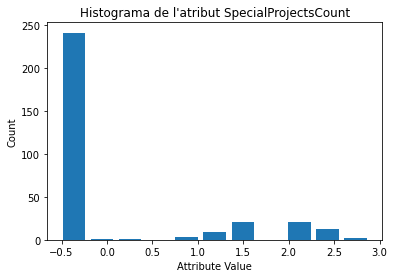
\includegraphics[width=0.3\textwidth]{HISTOGRAMAS/histograma_specialprojectscount.png}}
   \subfloat[\hspace{2 em}Termd]{
    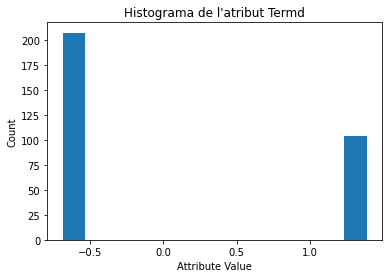
\includegraphics[width=0.3\textwidth]{HISTOGRAMAS/histograma_termd.png}}
  \subfloat[\hspace{2 em}TermReason]{
    \includegraphics[width=0.3\textwidth]{HISTOGRAMAS/histograma_termreason.png}}
\end{figure}
\begin{figure}[h]
\captionsetup[subfigure]{labelformat=empty}
\centering
\subfloat[\hspace{2 em}Zip]{
    \includegraphics[width=0.3\textwidth]{HISTOGRAMAS/histograma_zip.png}}
\end{figure}
\newpage

\subsection{PCA} \label{PCA}
\subsubsection{Representació 2 a 2 en R3}
Es mostra a continuació el conjunt total de gràfics que representen el Salary respecte a 2 atributs.\\\\
\textbf{IMPORTANT:} No s'ha vist necessària la creació de més gràfics amb l'ús d'altres atributs, ja que els representats són els que més relació tenen amb l'objectiu \textit{Salary}, per la qual s'analitza la tendència del salari usant únicament els més rellevants.

\begin{figure}[h]
\captionsetup[subfigure]{labelformat=empty}
\centering
  \subfloat[\hspace{2 em}DateofHire \& Department]{
    \includegraphics[width=0.5\textwidth]{pca/pca_dateofhire_department.png}}
  \subfloat[\hspace{2 em}DateofHire \& ManagerName]{
    \includegraphics[width=0.5\textwidth]{pca/pca_dateofhire_managername.png}}
\end{figure}    
\begin{figure}[h]
\captionsetup[subfigure]{labelformat=empty}
 \centering
 \subfloat[\hspace{2 em}DateofHire \& SpecialProjectsCount]{
    \includegraphics[width=0.5\textwidth]{pca/pca_dateofhire_specialprojects.png}}
  \subfloat[\hspace{2 em}Department \& ManagerName]{
    \includegraphics[width=0.5\textwidth]{pca/pca_department_managername.png}}
\end{figure}    
\newpage
\begin{figure}[h] 
 \centering
\captionsetup[subfigure]{labelformat=empty}
  \subfloat[\hspace{2 em}Position \& ManagerName]{
    \includegraphics[width=0.45\textwidth]{pca/pca_position_managername.png}}
  \subfloat[\hspace{2 em}Position \& SpecialProjectsCount]{
    \includegraphics[width=0.45\textwidth]{pca/pca_position_specialprojectscount.png}}
\end{figure}
\begin{figure}[h]
 \centering
\captionsetup[subfigure]{labelformat=empty}
 \subfloat[\hspace{2 em}Position \& DateofHire]{
    \includegraphics[width=0.45\textwidth]{pca/pca_position_dateofhire.png}}
  \subfloat[\hspace{2 em}Position \& Department]{
    \includegraphics[width=0.45\textwidth]{pca/pca_position_department.png}}
\end{figure}    
\begin{figure}[h]   
 \centering
\captionsetup[subfigure]{labelformat=empty}
\subfloat[\hspace{2 em}Department \& SpecialProjectsCount]{
    \includegraphics[width=0.45\textwidth]{pca/pca_department_specialprojectscount.png}}
  \subfloat[\hspace{2 em}ManagerName \& SpecialProjectsCount]{
    \includegraphics[width=0.45\textwidth]{pca/pca_managername_specialprojectscount.png}}
\end{figure} 
\newpage
\subsubsection{Representació 3 a 3 en R4} \label{Representació 3 a 3 en R4}
Es mostra a continuació el conjunt total de gràfics que representen el Salary respecte a 3 atributs.\\\\
\textbf{IMPORTANT:} No s'ha vist necessària la creació de més gràfics amb l'ús d'altres atributs, ja que els representats són els que més relació tenen amb l'objectiu \textit{Salary}, per la qual cosa s'analitza la tendència del salari usant únicament els més rellevants.

\begin{figure}[h]
\captionsetup[subfigure]{labelformat=empty}
 \centering
  \subfloat[\hspace{2 em}Position \& ManagerName]{
    \includegraphics[width=0.45\textwidth]{pca/pca_dateofhire_department_managername.png}}
  \subfloat[\hspace{2 em}Position \& SpecialProjectsCount]{
    \includegraphics[width=0.45\textwidth]{pca/pca_deparment_managername_special.png}}
\end{figure}
\begin{figure}[h]
\captionsetup[subfigure]{labelformat=empty}
 \centering
 \subfloat[\hspace{2 em}Position \& DateofHire]{
    \includegraphics[width=0.45\textwidth]{pca/pca_managername_special_position.png}}
  \subfloat[\hspace{2 em}Position \& Department]{
    \includegraphics[width=0.45\textwidth]{pca/pca_position_dateofhire_department.png}}
\end{figure}
\begin{figure}[h]
\captionsetup[subfigure]{labelformat=empty}
 \centering
 \subfloat[\hspace{2 em}Department \& SpecialProjectsCount]{
    \includegraphics[width=0.5\textwidth]{pca/pca_specialproject_position_dateofhire.png}}
\end{figure}
\subsection{Regressions}
\subsubsection{Regressor lineal simple}\label{graf_regresion}
\begin{figure}[h]
\captionsetup[subfigure]{labelformat=empty}
    \centering
    \subfloat[\hspace{2 em}Absences]{
    \subfloat[\hspace{2 em}MSE: 626540202.0400987]{
    \subfloat[\hspace{2 em}R2: 0.006786819677949918]{
    \includegraphics[width=0.5\textwidth]{lineal_std/lineal_std_absences.png}}}}
    \subfloat[\hspace{2 em}DateofHire]{
    \subfloat[\hspace{2 em}MSE: 414176096.7049033]{
    \subfloat[\hspace{2 em}R2: 0.3434337383583841]{
    \includegraphics[width=0.5\textwidth]{lineal_std/lineal_std_dateofhire.png}}}}
\end{figure}
\begin{figure}[h]
\captionsetup[subfigure]{labelformat=empty}
    \centering
    \subfloat[\hspace{2 em}DaysLate30]{
    \subfloat[\hspace{2 em}MSE: 627779473.6930523]{
    \subfloat[\hspace{2 em}R2:  0.004822283426795915]{
    \includegraphics[width=0.5\textwidth]{lineal_std/lineal_std_dayslast30.png}}}}
    \subfloat[\hspace{2 em}Department]{
    \subfloat[\hspace{2 em}MSE: 386909794.34377193]{
    \subfloat[\hspace{2 em}R2:  0.38665722313325035]{
    \includegraphics[width=0.5\textwidth]{lineal_std/lineal_std_department.png}}}}
\end{figure}
\newpage
\begin{figure}[h]
\captionsetup[subfigure]{labelformat=empty}
    \centering
    \subfloat[\hspace{2 em}DeptID]{
    \subfloat[\hspace{2 em}MSE: 504138517.07700574]{
    \subfloat[\hspace{2 em}R2:  0.20082220065289724]{
    \includegraphics[width=0.5\textwidth]{lineal_std/lineal_std_deptID.png}}}}
    \subfloat[\hspace{2 em}EmpID]{
    \subfloat[\hspace{2 em}MSE: 622432502.2573311]{
    \subfloat[\hspace{2 em}R2: 0.013298487327952357]{
    \includegraphics[width=0.5\textwidth]{lineal_std/lineal_std_empID.png}}}}
\end{figure}
\begin{figure}[h]
\captionsetup[subfigure]{labelformat=empty}
    \centering
    \subfloat[\hspace{2 em}EngagementSurvey]{
    \subfloat[\hspace{2 em}MSE: 628159034.582883]{
    \subfloat[\hspace{2 em}R2: 0.004220590387326029]{
    \includegraphics[width=0.5\textwidth]{lineal_std/lineal_std_engagement.png}}}}
    \subfloat[\hspace{2 em}LastPermanceReviewDate]{
    \subfloat[\hspace{2 em}MSE: 490471840.0394999]{
    \subfloat[\hspace{2 em}R2: 0.22248708938734219]{
    \includegraphics[width=0.5\textwidth]{lineal_std/lineal_std_lastperformance.png}}}}
\end{figure}
\newpage
\begin{figure}[h]
\captionsetup[subfigure]{labelformat=empty}
    \centering
    \subfloat[\hspace{2 em}Position]{
    \subfloat[\hspace{2 em}MSE: 100190785.86004275]{
    \subfloat[\hspace{2 em}R2: 0.8411741038500034]{
    \includegraphics[width=0.5\textwidth]{lineal_std/lineal_std_position.png}}}}
    \subfloat[\hspace{2 em}PositionID]{
    \subfloat[\hspace{2 em}MSE: 620067972.5629187]{
    \subfloat[\hspace{2 em}R2: 0.017046821513222787]{
    \includegraphics[width=0.5\textwidth]{lineal_std/lineal_std_positionID.png}}}}
\end{figure}
\begin{figure}[h]
\captionsetup[subfigure]{labelformat=empty}
    \centering
    \subfloat[\hspace{2 em}RaceDesc]{
    \subfloat[\hspace{2 em}MSE: 618409880.2199701]{
    \subfloat[\hspace{2 em}R2: 0.019675286795809654]{
    \includegraphics[width=0.5\textwidth]{lineal_std/lineal_std_racedesc.png}}}}
    \subfloat[\hspace{2 em}RecruitmentSource]{
    \subfloat[\hspace{2 em}MSE: 592443409.9534619]{
    \subfloat[\hspace{2 em}R2: 0.0608382328145336]{
    \includegraphics[width=0.5\textwidth]{lineal_std/lineal_std_recruitmentsource.png}}}}
\end{figure}
\newpage
\begin{figure}[h]
\captionsetup[subfigure]{labelformat=empty}
    \centering
    \subfloat[\hspace{2 em}ManagerID]{
    \subfloat[\hspace{2 em}MSE: 508907959.42527676]{
    \subfloat[\hspace{2 em}R2: 0.19326151581948225]{
    \includegraphics[width=0.5\textwidth]{lineal_std/lineal_std_managerid.png}}}}
    \subfloat[\hspace{2 em}ManagerName]{
    \subfloat[\hspace{2 em}MSE: 361109772.7375548]{
    \subfloat[\hspace{2 em}R2: 0.42755630898352837]{
    \includegraphics[width=0.5\textwidth]{lineal_std/lineal_std_managername.png}}}}
\end{figure}
\begin{figure}[h]
\captionsetup[subfigure]{labelformat=empty}
    \centering
    \subfloat[\hspace{2 em}SpecialProjectsCount]{
    \subfloat[\hspace{2 em}MSE: 467815729.6762194]{
    \subfloat[\hspace{2 em}R2: 0.25840233848767225]{
    \includegraphics[width=0.5\textwidth]{lineal_std/lineal_std_specialproject.png}}}}
    \subfloat[\hspace{2 em}State]{
    \subfloat[\hspace{2 em}MSE: 617328601.8822374]{
    \subfloat[\hspace{2 em}R2: 0.021389366583724256]{
    \includegraphics[width=0.5\textwidth]{lineal_std/lineal_std_state.png}}}}
\end{figure}
\newpage
\begin{figure}[h]
\captionsetup[subfigure]{labelformat=empty}
    \centering
    \subfloat[\hspace{2 em}Zip]{
    \subfloat[\hspace{2 em}MSE: 629946550.878149]{
    \subfloat[\hspace{2 em}R2: 0.0013869577828778956]{
    \includegraphics[width=0.5\textwidth]{lineal_std/lineal_std_zip.png}}}}
\end{figure}
\newpage
\subsubsection{Regressor lineal simple amb la transformació logarítmica}\label{regressio_lineal_simple_log}
\begin{figure}[h]
\captionsetup[subfigure]{labelformat=empty}
    \centering
    \subfloat[\hspace{2 em}Absences]{
    \subfloat[\hspace{2 em}MSE: 0.07525780628277791]{
    \subfloat[\hspace{2 em}R2: 0.006470672577135184]{
    \includegraphics[width=0.5\textwidth]{Regressor lineal logaritmo/logaritmica_absences.png}}}}
    \subfloat[\hspace{2 em}DateofHire]{
    \subfloat[\hspace{2 em}MSE: 0.045085675903278666]{
    \subfloat[\hspace{2 em}R2: 0.40479342317953737]{
    \includegraphics[width=0.5\textwidth]{Regressor lineal logaritmo/logaritmica_dateofhire.png}}}}
\end{figure}
\begin{figure}[h]
\captionsetup[subfigure]{labelformat=empty}
    \centering
    \subfloat[\hspace{2 em}DaysLate30]{
    \subfloat[\hspace{2 em}MSE: 0.07527435710257503]{
    \subfloat[\hspace{2 em}R2:  0.0062521739831206125]{
    \includegraphics[width=0.5\textwidth]{Regressor lineal logaritmo/logaritmica_dayslate30.png}}}}
    \subfloat[\hspace{2 em}Department]{
    \subfloat[\hspace{2 em}MSE: 0.04240950809387157]{
    \subfloat[\hspace{2 em}R2:  0.44012332894054845]{
    \includegraphics[width=0.5\textwidth]{Regressor lineal logaritmo/logaritmica_department.png}}}}
\end{figure}
\newpage
\begin{figure}[h]
\captionsetup[subfigure]{labelformat=empty}
    \centering
    \subfloat[\hspace{2 em}DeptID]{
    \subfloat[\hspace{2 em}MSE: 0.059223394919220095]{
    \subfloat[\hspace{2 em}R2:  0.21815180872131623]{
    \includegraphics[width=0.5\textwidth]{Regressor lineal logaritmo/logaritmica_deptID.png}}}}
    \subfloat[\hspace{2 em}EmpID]{
    \subfloat[\hspace{2 em}MSE: 0.07481253227632162]{
    \subfloat[\hspace{2 em}R2: 0.012349036643331424]{
    \includegraphics[width=0.5\textwidth]{Regressor lineal logaritmo/logaritmica_empID.png}}}}
\end{figure}
\begin{figure}[h]
\captionsetup[subfigure]{labelformat=empty}
    \centering
    \subfloat[\hspace{2 em}EngagementSurvey]{
    \subfloat[\hspace{2 em}MSE: 0.07550062787490819]{
    \subfloat[\hspace{2 em}R2: 0.0032650201002807355]{
    \includegraphics[width=0.5\textwidth]{Regressor lineal logaritmo/logaritmica_engagementsurvey.png}}}}
    \subfloat[\hspace{2 em}LastPermanceReviewDate]{
    \subfloat[\hspace{2 em}MSE: 0.053264597302605535]{
    \subfloat[\hspace{2 em}R2: 0.29681793627277564]{
    \includegraphics[width=0.5\textwidth]{Regressor lineal logaritmo/logaritmica_lastperformancereviewdate.png}}}}
\end{figure}
\newpage
\begin{figure}[h]
\captionsetup[subfigure]{labelformat=empty}
    \centering
    \subfloat[\hspace{2 em}Position]{
    \subfloat[\hspace{2 em}MSE:  0.010441290590750434]{
    \subfloat[\hspace{2 em}R2: 0.8621574434540897]{
    \includegraphics[width=0.5\textwidth]{Regressor lineal logaritmo/logaritmica_position.png}}}}
    \subfloat[\hspace{2 em}PositionID]{
    \subfloat[\hspace{2 em}MSE:  0.07453399781915082]{
    \subfloat[\hspace{2 em}R2:  0.016026158865804163]{
    \includegraphics[width=0.5\textwidth]{Regressor lineal logaritmo/logaritmica_positionID.png}}}}
\end{figure}
\begin{figure}[h]
\captionsetup[subfigure]{labelformat=empty}
    \centering
    \subfloat[\hspace{2 em}RaceDesc]{
    \subfloat[\hspace{2 em}MSE:  0.0740237234378234]{
    \subfloat[\hspace{2 em}R2:  0.022762636952561865]{
    \includegraphics[width=0.5\textwidth]{Regressor lineal logaritmo/logaritmica_raceDesc.png}}}}
    \subfloat[\hspace{2 em}RecruitmentSource]{
    \subfloat[\hspace{2 em}MSE:  0.07027300405067168]{
    \subfloat[\hspace{2 em}R2:  0.07227842666435225]{
    \includegraphics[width=0.5\textwidth]{Regressor lineal logaritmo/logaritmica_recruitmentsource.png}}}}
\end{figure}
\newpage
\begin{figure}[h]
\captionsetup[subfigure]{labelformat=empty}
    \centering
    \subfloat[\hspace{2 em}ManagerID]{
    \subfloat[\hspace{2 em}MSE:  0.05839603299804237]{
    \subfloat[\hspace{2 em}R2:  0.2290743744149576]{
    \includegraphics[width=0.5\textwidth]{Regressor lineal logaritmo/logaritmica_managerID.png}}}}
    \subfloat[\hspace{2 em}ManagerName]{
    \subfloat[\hspace{2 em}MSE:  0.03635255366889941]{
    \subfloat[\hspace{2 em}R2:  0.5200852910719191]{
    \includegraphics[width=0.5\textwidth]{Regressor lineal logaritmo/logaritmica_managername.png}}}}
\end{figure}
\begin{figure}[h]
\captionsetup[subfigure]{labelformat=empty}
    \centering
    \subfloat[\hspace{2 em}SpecialProjectsCount]{
    \subfloat[\hspace{2 em}MSE:  0.05137053026138132]{
    \subfloat[\hspace{2 em}R2:  0.32182279950902926]{
    \includegraphics[width=0.5\textwidth]{Regressor lineal logaritmo/logaritmica_specialprojectscount.png}}}}
    \subfloat[\hspace{2 em}State]{
    \subfloat[\hspace{2 em}MSE:  0.07376241895106724]{
    \subfloat[\hspace{2 em}R2:  0.026212294653237267]{
    \includegraphics[width=0.5\textwidth]{Regressor lineal logaritmo/logaritmica_state.png}}}}
\end{figure}
\newpage
\begin{figure}[h]
\captionsetup[subfigure]{labelformat=empty}
    \centering
    \subfloat[\hspace{2 em}Zip]{
    \subfloat[\hspace{2 em}MSE: 0.0757306982506967]{
    \subfloat[\hspace{2 em}R2:  0.00022770507600045065]{
    \includegraphics[width=0.5\textwidth]{Regressor lineal logaritmo/logaritmica_zip.png}}}}
\end{figure}
\newpage
\subsubsection{Lasso amb la transformació logarítmica}
\begin{figure}[h]
\captionsetup[subfigure]{labelformat=empty}
    \centering
    \subfloat[\hspace{2 em}Absences]{
    \subfloat[\hspace{2 em}MSE: 0.07525880950858431]{
    \subfloat[\hspace{2 em}R2: 0.0064574283130519605]{
    \includegraphics[width=0.5\textwidth]{lasso/log_laso_absences.png}}}}
    \subfloat[\hspace{2 em}DateofHire]{
    \subfloat[\hspace{2 em}MSE: 0.04508667912908511]{
    \subfloat[\hspace{2 em}R2: 0.40478017891545426]{
    \includegraphics[width=0.5\textwidth]{lasso/log_laso_dateofhire.png}}}}
\end{figure}
\begin{figure}[h]
\captionsetup[subfigure]{labelformat=empty}
    \centering
    \subfloat[\hspace{2 em}DaysLate30]{
    \subfloat[\hspace{2 em}MSE: 0.07527536032838153]{
    \subfloat[\hspace{2 em}R2:  0.006238929719037611]{
    \includegraphics[width=0.5\textwidth]{lasso/log_laso_dayslate30.png}}}}
    \subfloat[\hspace{2 em}Department]{
    \subfloat[\hspace{2 em}MSE: 0.042410511319678004]{
    \subfloat[\hspace{2 em}R2:  0.4401100846764652]{
    \includegraphics[width=0.5\textwidth]{lasso/log_laso_department.png}}}}
\end{figure}
\newpage
\begin{figure}[h]
\captionsetup[subfigure]{labelformat=empty}
    \centering
    \subfloat[\hspace{2 em}DeptID]{
    \subfloat[\hspace{2 em}MSE: 0.0592243981450266]{
    \subfloat[\hspace{2 em}R2:  0.21813856445723245]{
    \includegraphics[width=0.5\textwidth]{lasso/log_laso_deptID.png}}}}
    \subfloat[\hspace{2 em}EmpID]{
    \subfloat[\hspace{2 em}MSE: 0.07481353550212792]{
    \subfloat[\hspace{2 em}R2: 0.012335792379248534]{
    \includegraphics[width=0.5\textwidth]{lasso/log_laso_empID.png}}}}
\end{figure}
\begin{figure}[h]
\captionsetup[subfigure]{labelformat=empty}
    \centering
    \subfloat[\hspace{2 em}EngagementSurvey]{
    \subfloat[\hspace{2 em}MSE: 0.07550163110071467]{
    \subfloat[\hspace{2 em}R2: 0.0032517758361974014]{
    \includegraphics[width=0.5\textwidth]{lasso/log_laso_engagementsurvey.png}}}}
    \subfloat[\hspace{2 em}LastPerformanceReviewDate]{
    \subfloat[\hspace{2 em}MSE: 0.053265600528411984]{
    \subfloat[\hspace{2 em}R2: 0.2968046920086922]{
    \includegraphics[width=0.5\textwidth]{lasso/log_laso_lasperformancereviewdate.png}}}}
\end{figure}
\newpage
\begin{figure}[h]
\captionsetup[subfigure]{labelformat=empty}
    \centering
    \subfloat[\hspace{2 em}Position]{
    \subfloat[\hspace{2 em}MSE:  0.010442293816556885]{
    \subfloat[\hspace{2 em}R2: 0.8621441991900065]{
    \includegraphics[width=0.5\textwidth]{lasso/log_laso_position.png}}}}
    \subfloat[\hspace{2 em}PositionID]{
    \subfloat[\hspace{2 em}MSE:  0.07453500104495724]{
    \subfloat[\hspace{2 em}R2:  0.016012914601721162]{
    \includegraphics[width=0.5\textwidth]{lasso/log_laso_positionID.png}}}}
\end{figure}
\begin{figure}[h]
\captionsetup[subfigure]{labelformat=empty}
    \centering
    \subfloat[\hspace{2 em}RaceDesc]{
    \subfloat[\hspace{2 em}MSE: 0.07402472666362968]{
    \subfloat[\hspace{2 em}R2: 0.02274939268847842]{
    \includegraphics[width=0.5\textwidth]{lasso/log_laso_racedesc.png}}}}
    \subfloat[\hspace{2 em}RecruitmentSource]{
    \subfloat[\hspace{2 em}MSE: 0.07027400727647805]{
    \subfloat[\hspace{2 em}R2: 0.07226518240026925]{
    \includegraphics[width=0.5\textwidth]{lasso/log_laso_recruitmentscore.png}}}}
\end{figure}
\newpage
\begin{figure}[h]
\captionsetup[subfigure]{labelformat=empty}
    \centering
    \subfloat[\hspace{2 em}SpecialProjectsCount]{
    \subfloat[\hspace{2 em}MSE: 0.05137153348718776]{
    \subfloat[\hspace{2 em}R2: 0.3218095552449459]{
    \includegraphics[width=0.5\textwidth]{lasso/log_laso_specialprojectscount.png}}}}
    \subfloat[\hspace{2 em}State]{
    \subfloat[\hspace{2 em}MSE: 0.07376342217687368]{
    \subfloat[\hspace{2 em}R2: 0.026199050389153933]{
    \includegraphics[width=0.5\textwidth]{lasso/log_laso_state.png}}}}
\end{figure}
\begin{figure}[h]
\captionsetup[subfigure]{labelformat=empty}
    \centering
    \subfloat[\hspace{2 em}ManagerID]{
    \subfloat[\hspace{2 em}MSE: 0.058397036223848835]{
    \subfloat[\hspace{2 em}R2: 0.22906113015087393]{
    \includegraphics[width=0.5\textwidth]{lasso/log_laso_managerid.png}}}}
    \subfloat[\hspace{2 em}ManagerName]{
    \subfloat[\hspace{2 em}MSE: 0.036353556894705874]{
    \subfloat[\hspace{2 em}R2: 0.520072046807836]{
    \includegraphics[width=0.5\textwidth]{lasso/log_laso_managername.png}}}}
\end{figure}

\newpage
\begin{figure}[h]
\captionsetup[subfigure]{labelformat=empty}
    \centering
    \subfloat[\hspace{2 em}Zip]{
    \subfloat[\hspace{2 em}MSE: 0.0757317014765031]{
    \subfloat[\hspace{2 em}R2: 0.00021446081191722755]{
    \includegraphics[width=0.5\textwidth]{lasso/log_laso_zip.ong.png}}}}
\end{figure}
\newpage
\subsubsection{BayessianRidge amb la transformació logarítmica}
\begin{figure}[h]
\captionsetup[subfigure]{labelformat=empty}
    \centering
    \subfloat[\hspace{2 em}Absences]{
    \subfloat[\hspace{2 em}MSE: 0.07537440201438339]{
    \subfloat[\hspace{2 em}R2: 0.004931413269374962]{
    \includegraphics[width=0.5\textwidth]{bayes/log_bayes_absences.png}}}}
    \subfloat[\hspace{2 em}DateofHire]{
    \subfloat[\hspace{2 em}MSE: 0.045086365657429864]{
    \subfloat[\hspace{2 em}R2: 0.40478431726731656]{
    \includegraphics[width=0.5\textwidth]{bayes/log_bayes_dateofhire.png}}}}
\end{figure}
\begin{figure}[h]
\captionsetup[subfigure]{labelformat=empty}
    \centering
    \subfloat[\hspace{2 em}DaysLate30]{
    \subfloat[\hspace{2 em}MSE: 0.0753946963498982]{
    \subfloat[\hspace{2 em}R2:  0.004663493986173828]{
    \includegraphics[width=0.5\textwidth]{bayes/log_bayes_dayslatelast30.png}}}}
    \subfloat[\hspace{2 em}Department]{
    \subfloat[\hspace{2 em}MSE: 0.04241006940975646]{
    \subfloat[\hspace{2 em}R2:  0.44011591862896604]{
    \includegraphics[width=0.5\textwidth]{bayes/log_bayes_department.png}}}}
\end{figure}
\newpage
\begin{figure}[h]
\captionsetup[subfigure]{labelformat=empty}
    \centering
    \subfloat[\hspace{2 em}DeptID]{
    \subfloat[\hspace{2 em}MSE: 0.059225603066942224]{
    \subfloat[\hspace{2 em}R2: 0.2181226574660562]{
    \includegraphics[width=0.5\textwidth]{bayes/log_bayes_deptid.png}}}}
    \subfloat[\hspace{2 em}EmpID]{
    \subfloat[\hspace{2 em}MSE: 0.07487431602134785]{
    \subfloat[\hspace{2 em}R2: 0.011533387534307327]{
    \includegraphics[width=0.5\textwidth]{bayes/log_bayes_empid.png}}}}
\end{figure}
\begin{figure}[h]
\captionsetup[subfigure]{labelformat=empty}
    \centering
    \subfloat[\hspace{2 em}EngagementSurvey]{
    \subfloat[\hspace{2 em}MSE: 0.07566204569408011]{
    \subfloat[\hspace{2 em}R2: 0.001134034024054098]{
    \includegraphics[width=0.5\textwidth]{bayes/log_bayes_engagementsurvey.png}}}}
    \subfloat[\hspace{2 em}LastPerformanceReviewDate]{
    \subfloat[\hspace{2 em}MSE: 0.05326591015695642]{
    \subfloat[\hspace{2 em}R2: 0.29680060439234135]{
    \includegraphics[width=0.5\textwidth]{bayes/log_bayes_lastperformancereviewdate.png}}}}
\end{figure}
\newpage
\begin{figure}[h]
\captionsetup[subfigure]{labelformat=empty}
    \centering
    \subfloat[\hspace{2 em}Position]{
    \subfloat[\hspace{2 em}MSE: 0.010441307960887996]{
    \subfloat[\hspace{2 em}R2: 0.8621572141391264]{
    \includegraphics[width=0.5\textwidth]{bayes/log_bayes_position.png}}}}
    \subfloat[\hspace{2 em}PositionID]{
    \subfloat[\hspace{2 em}MSE: 0.07458137547618211]{
    \subfloat[\hspace{2 em}R2: 0.01540069429209201]{
    \includegraphics[width=0.5\textwidth]{bayes/log_bayes_positionid.png}}}}
\end{figure}
\begin{figure}[h]
\captionsetup[subfigure]{labelformat=empty}
    \centering
    \subfloat[\hspace{2 em}RaceDesc]{
    \subfloat[\hspace{2 em}MSE: 0.07405669011226543]{
    \subfloat[\hspace{2 em}R2: 0.0223274215310183]{
    \includegraphics[width=0.5\textwidth]{bayes/log_bayes_racedesc.png}}}}
    \subfloat[\hspace{2 em}RecruitmentSource]{
    \subfloat[\hspace{2 em}MSE: 0.07028238251713365]{
    \subfloat[\hspace{2 em}R2: 0.07215461516975186]{
    \includegraphics[width=0.5\textwidth]{bayes/log_bayes_recruitmentsource.png}}}}
\end{figure}
\newpage
\begin{figure}[h]
\captionsetup[subfigure]{labelformat=empty}
    \centering
    \subfloat[\hspace{2 em}SpecialProjectsCount]{
    \subfloat[\hspace{2 em}MSE: 0.051371656542706694]{
    \subfloat[\hspace{2 em}R2: 0.32180793070560587]{
    \includegraphics[width=0.5\textwidth]{bayes/log_bayes_specialprojectcount.png}}}}
    \subfloat[\hspace{2 em}State]{
    \subfloat[\hspace{2 em}MSE: 0.07379086015554037]{
    \subfloat[\hspace{2 em}R2: 0.02583682302913648]{
    \includegraphics[width=0.5\textwidth]{bayes/log_bayes_state.png}}}}
\end{figure}
\begin{figure}[h]
\captionsetup[subfigure]{labelformat=empty}
    \centering
    \subfloat[\hspace{2 em}ManagerID]{
    \subfloat[\hspace{2 em}MSE: 0.058398077538854835]{
    \subfloat[\hspace{2 em}R2: 0.22904738304544214]{
    \includegraphics[width=0.5\textwidth]{bayes/log_bayes_managerid.png}}}}
    \subfloat[\hspace{2 em}ManagerName]{
    \subfloat[\hspace{2 em}MSE: 0.03635290269563891]{
    \subfloat[\hspace{2 em}R2: 0.5200806833332823]{
    \includegraphics[width=0.5\textwidth]{bayes/log_bayes_managername.png}}}}
\end{figure}

\newpage
\begin{figure}[h]
\captionsetup[subfigure]{labelformat=empty}
    \centering
    \subfloat[\hspace{2 em}Zip]{
    \subfloat[\hspace{2 em}MSE: 0.07574500493307051]{
    \subfloat[\hspace{2 em}R2: 3.883286169337197e-05]{
    \includegraphics[width=0.5\textwidth]{bayes/log_bayes_zip.png}}}}
\end{figure}


\newpage
\subsubsection{Regressió multilineal} \label{reg_multi}
Mostra del output del programa, per a l'output complet consultar el codi adjuntat.

\begin{verbatim}
['Position', 'DateofHire']
Mean squeared error:  105404799.54876395
R2 score:  0.8275056871982004
Coef:  [22235.6976501  1297.9132474]
Intercept:  69017.36571365858
--------------------------------------

            [···]

--------------------------------------
['Position', 'DateofHire', 'Department', 'ManagerName', 'SpecialProjectsCount']
Mean squeared error:  121985220.57901783
R2 score:  0.8046125176646411
Coef:  [23734.74740658  1958.13126168  2013.75626643 -2378.93585933
 -2685.22514853]
Intercept:  68977.85317116327
--------------------------------------
MILLOR R2 SCORE A:  ['Position', 'DateofHire', 'ManagerName'] 0.8275600914537563
MILLOR ERROR A:  ['Position', 'DateofHire', 'ManagerName', 'SpecialProjectsCount'] 
                 102709332.28481683
\end{verbatim}
\subsubsection{Regressió multilineal amb transformació logarítmica} \label{reg_multi_log}
Mostra del output del programa, per a l'output complet consultar el codi adjuntat.

\begin{verbatim}
['Position', 'DateofHire']
Mean squeared error:  0.010022008910896293
R2 score:  0.8563943243144865
Coef:  [0.23590029 0.03308796]
Intercept:  11.097657857934589
--------------------------------------

            [···]

--------------------------------------
['Position', 'DateofHire', 'Department', 'ManagerName', 'SpecialProjectsCount']
Mean squeared error:  0.010532039539133566
R2 score:  0.8501786812730818
Coef:  [ 0.23628708  0.03340143 -0.02047883  0.01055037  0.00918509]
Intercept:  11.097395616323494
--------------------------------------
MILLOR R2 SCORE A:  ['Position', 'DateofHire', 'ManagerName'] 0.8575794932710843
MILLOR ERROR A:  ['Position', 'DateofHire'] 0.010022008910896293    
\end{verbatim}
\newpage
\subsubsection{Lasso multilineal amb transformació logarítmica}\label{reg_multi_lasso}
Mostra del output del programa, per a l'output complet consultar el codi adjuntat.
\begin{verbatim}
['Position', 'DateofHire']
Mean squeared error:  0.021452992310037416
R2 score:  0.7132818071734579
Coef:  [0.15511766 0.        ]
Intercept:  11.097741043347556
--------------------------------------

            [···]

--------------------------------------
['Position', 'DateofHire', 'Department', 'ManagerName', 'SpecialProjectsCount']
Mean squeared error:  0.021220503098127275
R2 score:  0.7122942881409924
Coef:  [0.15546191 0.         0.         0.         0.        ]
Intercept:  11.097674174726995
--------------------------------------
MILLOR R2 SCORE A:  ['Position', 'DateofHire', 'ManagerName'] 
                    0.7162151968345063
MILLOR ERROR A:  ['Position', 'DateofHire', 'Department', 'ManagerName']
                 0.020889003305314513
\end{verbatim}
\subsubsection{BayessianRidge multilineal amb transformació logarítmica} \label{reg_multi_bay}
Mostra del output del programa, per a l'output complet consultar el codi adjuntat.
\begin{verbatim}
['Position', 'DateofHire']
Mean squeared error:  0.010032885386522068
R2 score:  0.8579434816618091
Coef:  [0.23555831 0.03324445]
Intercept:  11.097708518996102
--------------------------------------

            [···]

--------------------------------------
['Position', 'DateofHire', 'Department', 'ManagerName', 'SpecialProjectsCount']
Mean squeared error:  0.010398309068287022
R2 score:  0.8512454410542898
Coef:  [ 0.23426653  0.03370605 -0.016519    0.01062965  0.00639307]
Intercept:  11.097525592309028
--------------------------------------
MILLOR R2 SCORE A:  ['Position', 'DateofHire'] 0.8579434816618091
MILLOR ERROR A:  ['Position', 'DateofHire'] 0.010032885386522068
\end{verbatim}
\newpage
\subsection{Descens del gradient}\label{descens_gradient}
\begin{figure}[h]
    \centering
    \includegraphics[width = 0.7 \textwidth]{R2_GD.png}
    \caption{Primer exemple del regresor lineal programat amb un dataset aleatòri}
\end{figure}
\begin{figure}[h]
    \centering
    \includegraphics[width = 0.8 \textwidth]{R3_GD.png}
    \caption{Segon exemple del regresor lineal programat amb un dataset aleatori}
\end{figure}

\end{document}
